\section{L'area di studio: il Tagliamento}
\label{sec:descr-area-studio}
\paragraph{Inquadramento}
Nei fiumi a morfologia intrecciata dove l'impatto antropico non è intenso è possibile trovare isole nell'alveo dove il disturbo indotto dalle piene non è eccessivo;
queste si formano e accrescono nel periodo compreso tra eventi di piena di una certa entità, mentre vengono erose dagli eventi idrologici sufficientemente intensi \squarecites{Poff:1997}{Gurnell:2001-island-formation}.
La presenza delle isole ha un importante ruolo ecologico: la varietà spaziale e temporale di ambienti presenti (pozze d'acqua, sorgenti e canali separati da aridi sedimenti, zone con vegetazione bassa e rada alternate con isole fitte e mature che si modificano tra e in seguito alle piene) crea un mosaico in continuo cambiamento che sostiene una forte biodiversità \squarecites{Arscott:2002-habitat-dynamics}.
Inoltre, durante piene di piccola entità le piante influenzano l'accrescimento delle forme fluviali attraverso la ritenzione di sedimenti e materiale legnoso sia morto che vivo, inducendo così la successiva colonizzazione da parte di altre piante e la rimodellazione dei canali \squarecite{Gurnell:2006-omega}.


Il Fiume Tagliamento, situato nel Nord-Est italiano, è uno dei pochi fiumi alpini allo stato quasi naturale che presenta queste caratteristiche. 
Sono stati effettuati interventi di ingegneria fluviale, come arginature, derivazioni, pennelli, estrazione di ghiaia, sia in tratti posti a monte che in altri posti a valle; la loro entità è comunque tanto limitata da poter parlare di “contesto non gestito”.
\\
Difatti il Tagliamento presenta un regime idrologico non alterato, con piene frequenti ed imprevedibili dovute all'alta piovosità nel bacino \squarecites{Mosetti:1983}{Bertoldi:2009-2m} e alla limitata presenza di bacini di regolazione (solo il \SI{3}{\percent} dell'area drenante del bacino è intercettata da dighe \squarecite{Sitzia:2016-d50});
è stato suggerito che è possibile formulare previsioni accurate di un evento di piena solamente nelle 5 ore precedenti \squarecite{Arscott:2002-habitat-dynamics}. 
Inoltre, le sponde e l'alveo sono colonizzate da ampie porzioni di vegetazione riparia lungo quasi tutto il suo corso. 
Questi fatti indicano che le attività umane sul Tagliamento non sono tali da aver alterato o da alterare il regime del fiume.

Il bacino idrografico del Tagliamento, ampio circa~\SI{2900}{\kilo\m\tothe{2}}, si estende tra le province di Belluno, Udine, Pordenone e Venezia.
Il suo corso di circa~\SI{170}{\kilo\m} presenta morfologia intrecciata (\emph{braided}) con canali multipli separati da barre e isole.
Nelle parti montane è confinato dai versanti; 
nella parte planiziale è libero, con tratti larghi diverse centinaia di metri, se non più di \SI{1}{\kilo\m};
a qualche decina di chilometri dalla foce il fiume si restringe assumendo prima una forma transizionale monocursale con larghezza sui \SIrange[range-phrase={-}]{300}{200}{\m} nei pressi di Madrisio~(UD);
infine diventa meandriforme a Latisana~(UD) (larghezza intorno ai \SI{100}{\m}) fino alla foce, situata tra Bibione~(VE) e Lignano~(UD).
\\
Insieme alla variazione della morfologia del fiume si assiste ad un cambiamento nella granulometria: mentre la ghiaia predomina nella parte intrecciata ($d_{50} = \SI{4}{\centi\m}$ \squarecites{Bertoldi:2010-d50}{Sitzia:2016-d50}), a partire dal tratto meandriforme si trova solo sabbia sul fondo.
Questo mutamento di materiale trasportato riflette la riduzione della pendenza che si osserva dal tratto transizionale monocursale e che giustifica il passaggio da fiume “in ghiaia” a fiume “in sabbia”.
\\
Le precipitazioni sono mediamente di circa \SI{2000}{\mm} all'anno con forti variazioni locali; i minimi di precipitazione si registrano durante l'inverno, mentre i massimi in primavera e in autunno.
Si assiste anche ad eventi di breve durata e particolarmente intensi.
Il regime fluviale che ne risulta è di tipo \emph{flashy} pluvio-nivale con piene brevi ed intense così come piene di diversi giorni di durata.

Il tratto studiato è quello intrecciato multicanale compreso tra Tolmezzo~(UD) e Madrisio~(UD) (\cref{fig:overview,fig:overview-sat}). 
%
\begin{figure}
	\centering
	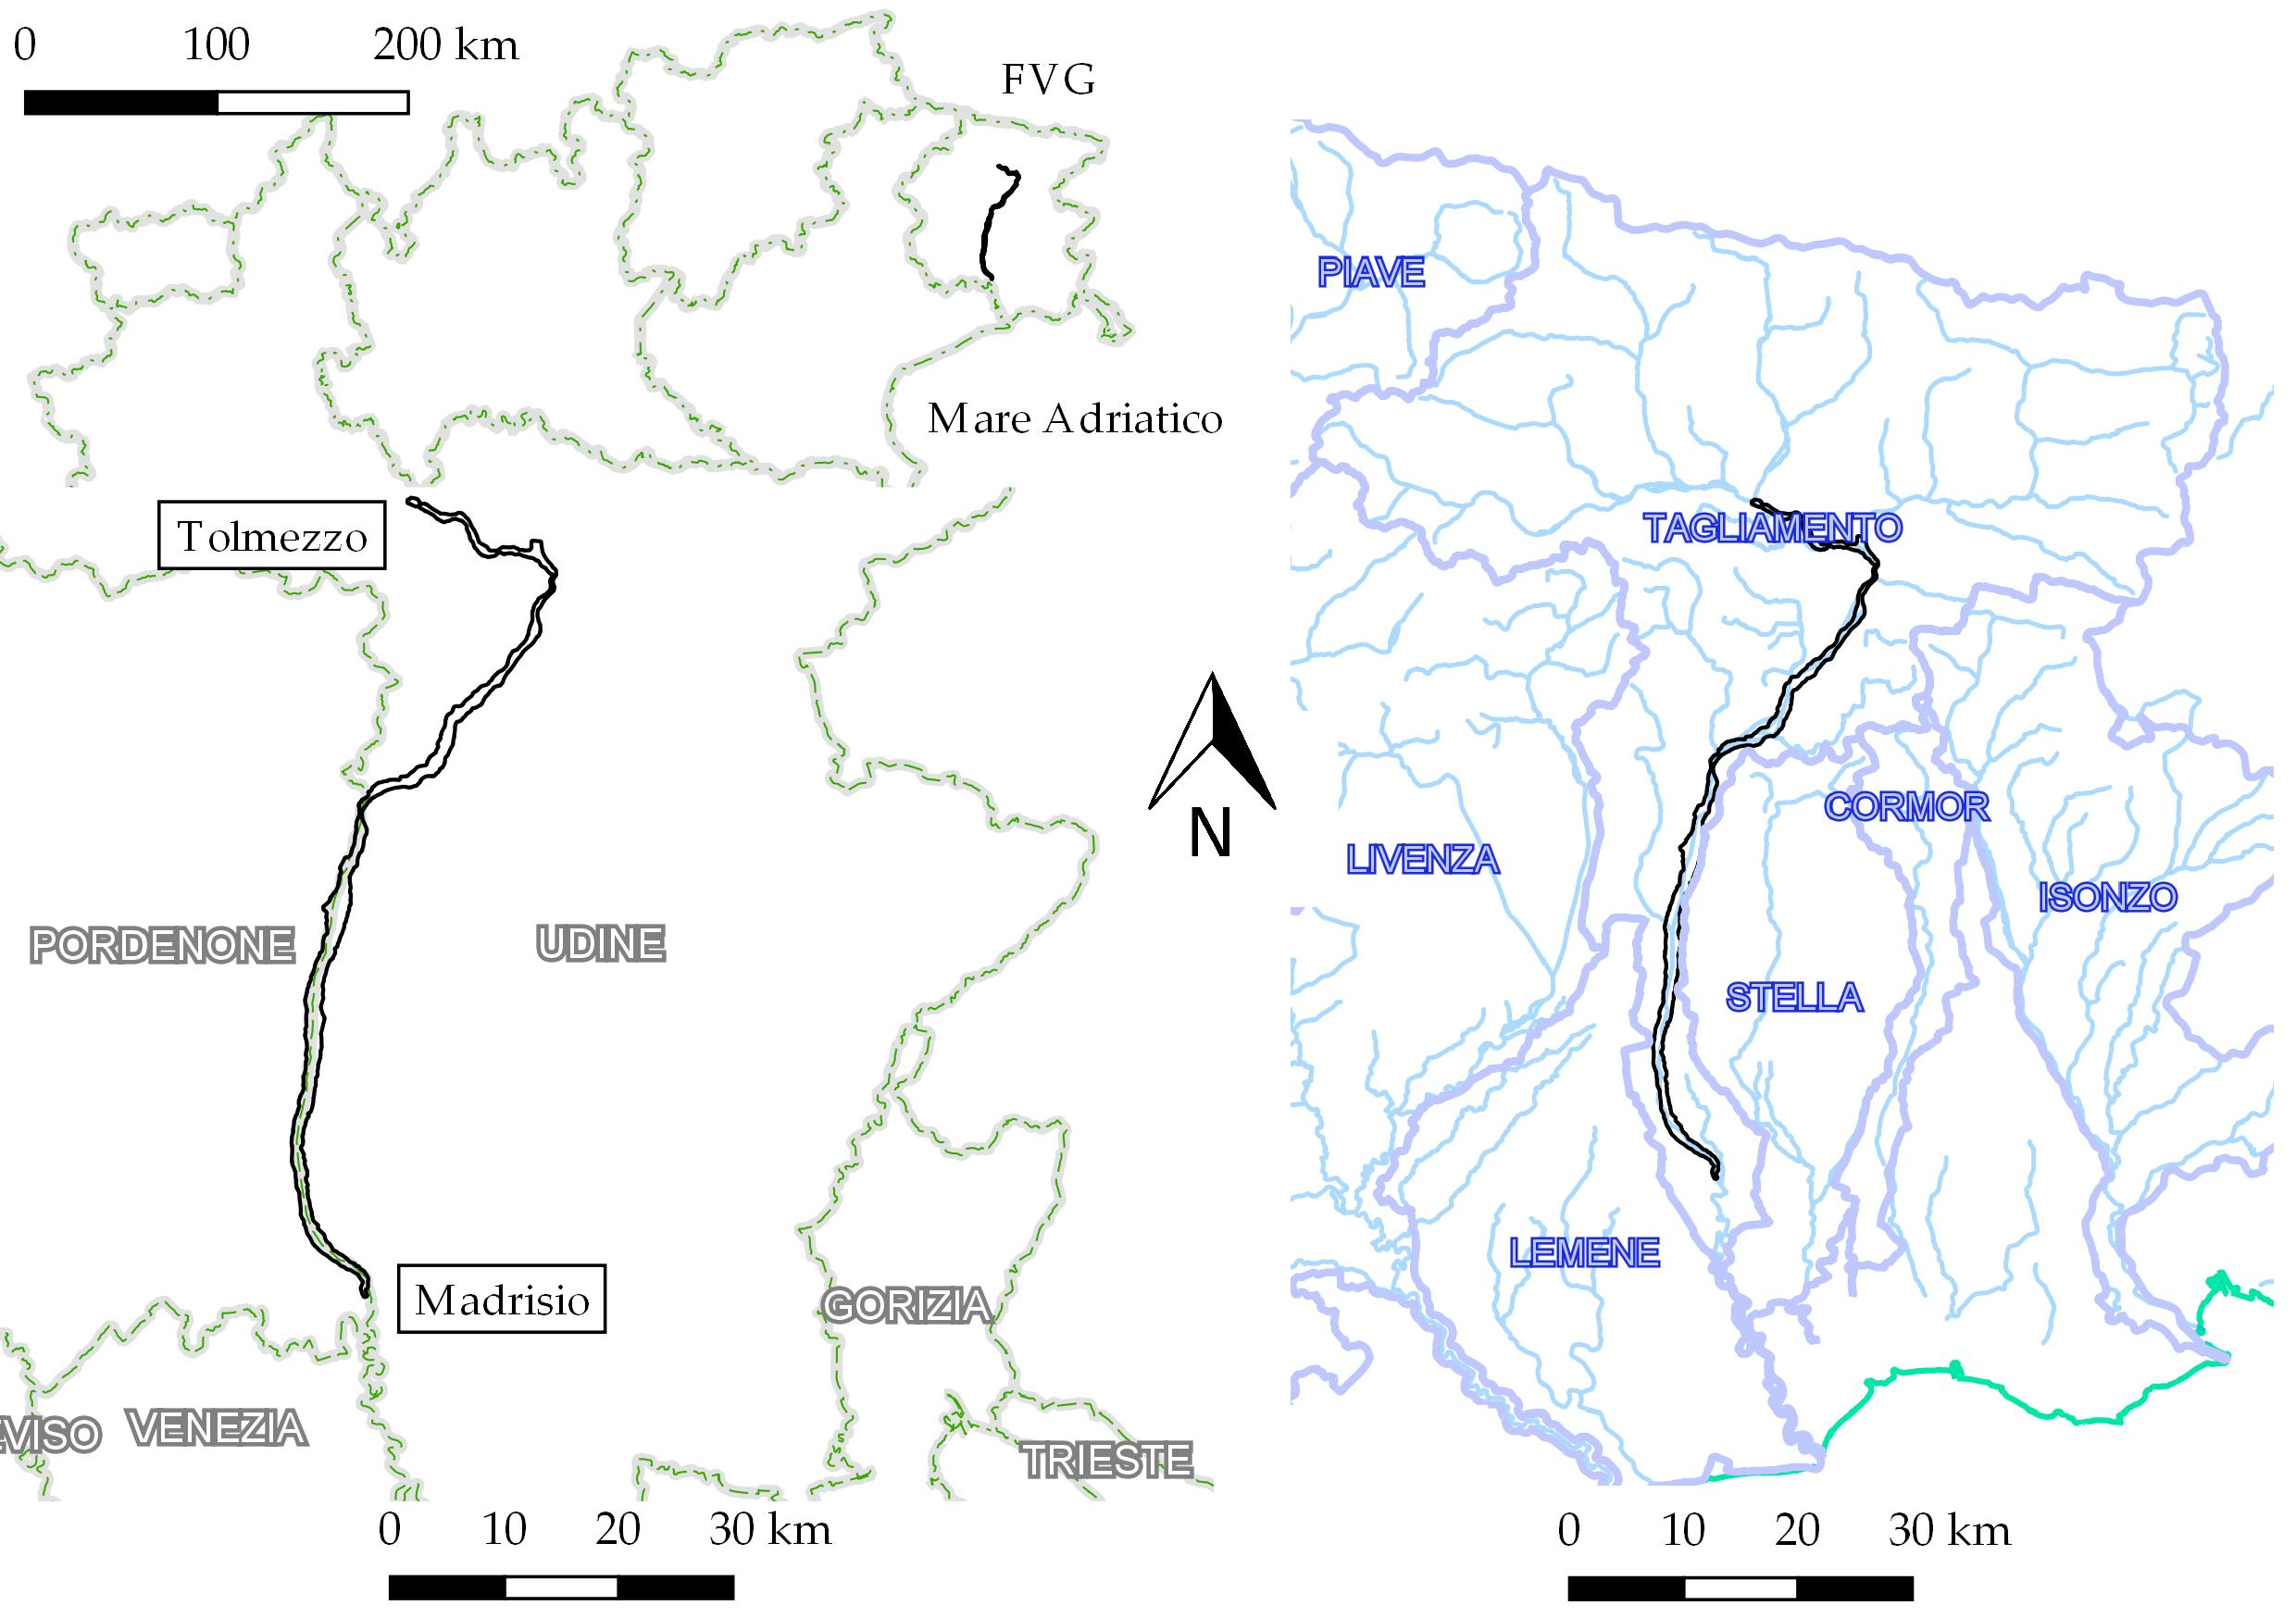
\includegraphics[width=\textwidth]{files/overview.jpeg}
	\caption[inquadramento dell'area di studio]
		{inquadramento dell'area di studio (poligono nero); a sinistra è mostrata l'Italia settentrionale (in alto) e un ingrandimento delle province e degli estremi dell'area di studio (in basso); a destra si vede il bacino idrografico del Tagliamento e di altri fiumi nelle vicinanze (in blu), il reticolo idrografico (in azzurro) e la linea di costa (in verde acqua). I tematismi provengono dal Portale Cartografico Nazionale del Ministero dell'Ambiente.}
	\label{fig:overview}
\end{figure}
%
\begin{figure}
	\centering
	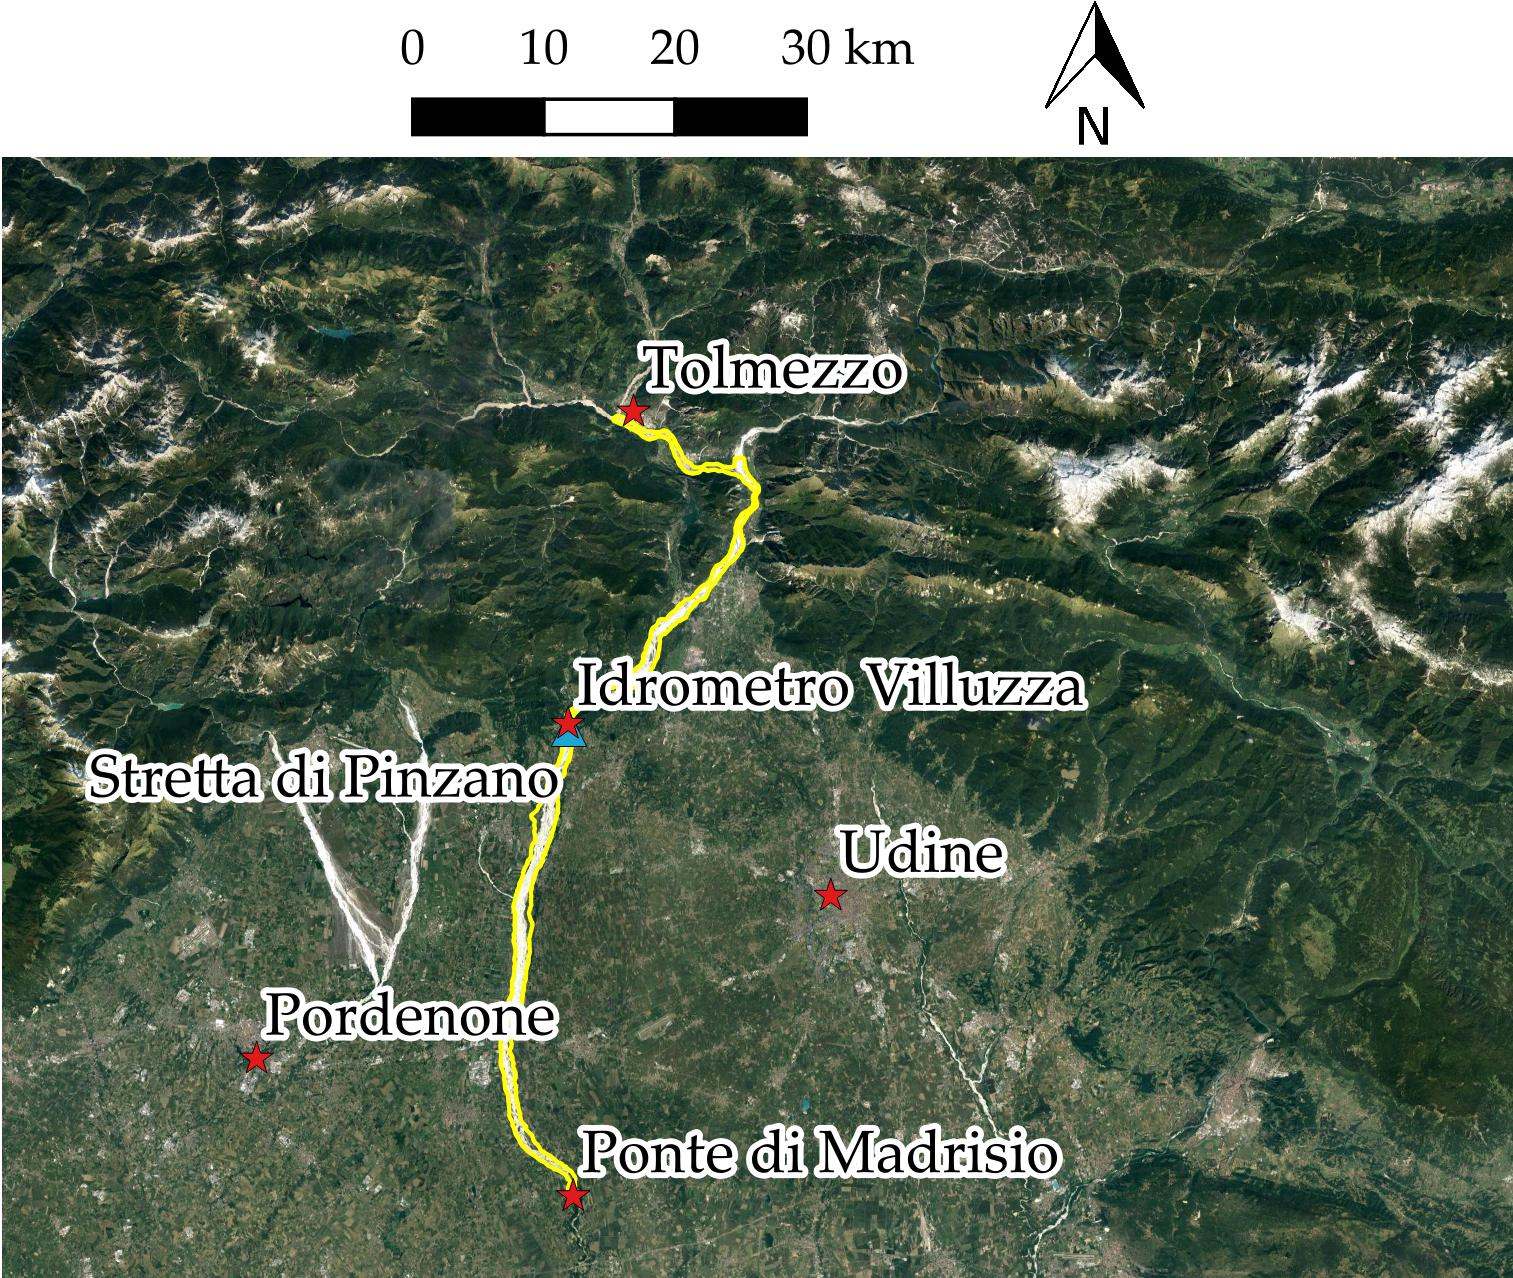
\includegraphics[width=\textwidth]{files/overview_tratto_sat.jpeg}
	\caption[inquadramento dell'area di studio]{inquadramento dell'area di studio (contornata in giallo).
	\\
	Map data: Google, Digital Globe.}
	\label{fig:overview-sat}
\end{figure}
%
\\
L'area di studio è stata suddivisa manualmente in 23~tratti al fine di avere un maggior dettaglio spaziale delle dinamiche di vegetazione (\cref{fig:23-tratti}). 
Questi tratti sono stati selezionati in modo da possedere caratteristiche omogenee per portata e crescita della vegetazione; 
pertanto confluenze di immissari, bruschi restringimenti o allargamenti, inizio di pronunciato \emph{upwelling} o \emph{downwelling} ed evidenti cambiamenti di morfologia fluviale sono stati gli elementi per individuare i 23~tratti.
%
\begin{figure}
	\centering
	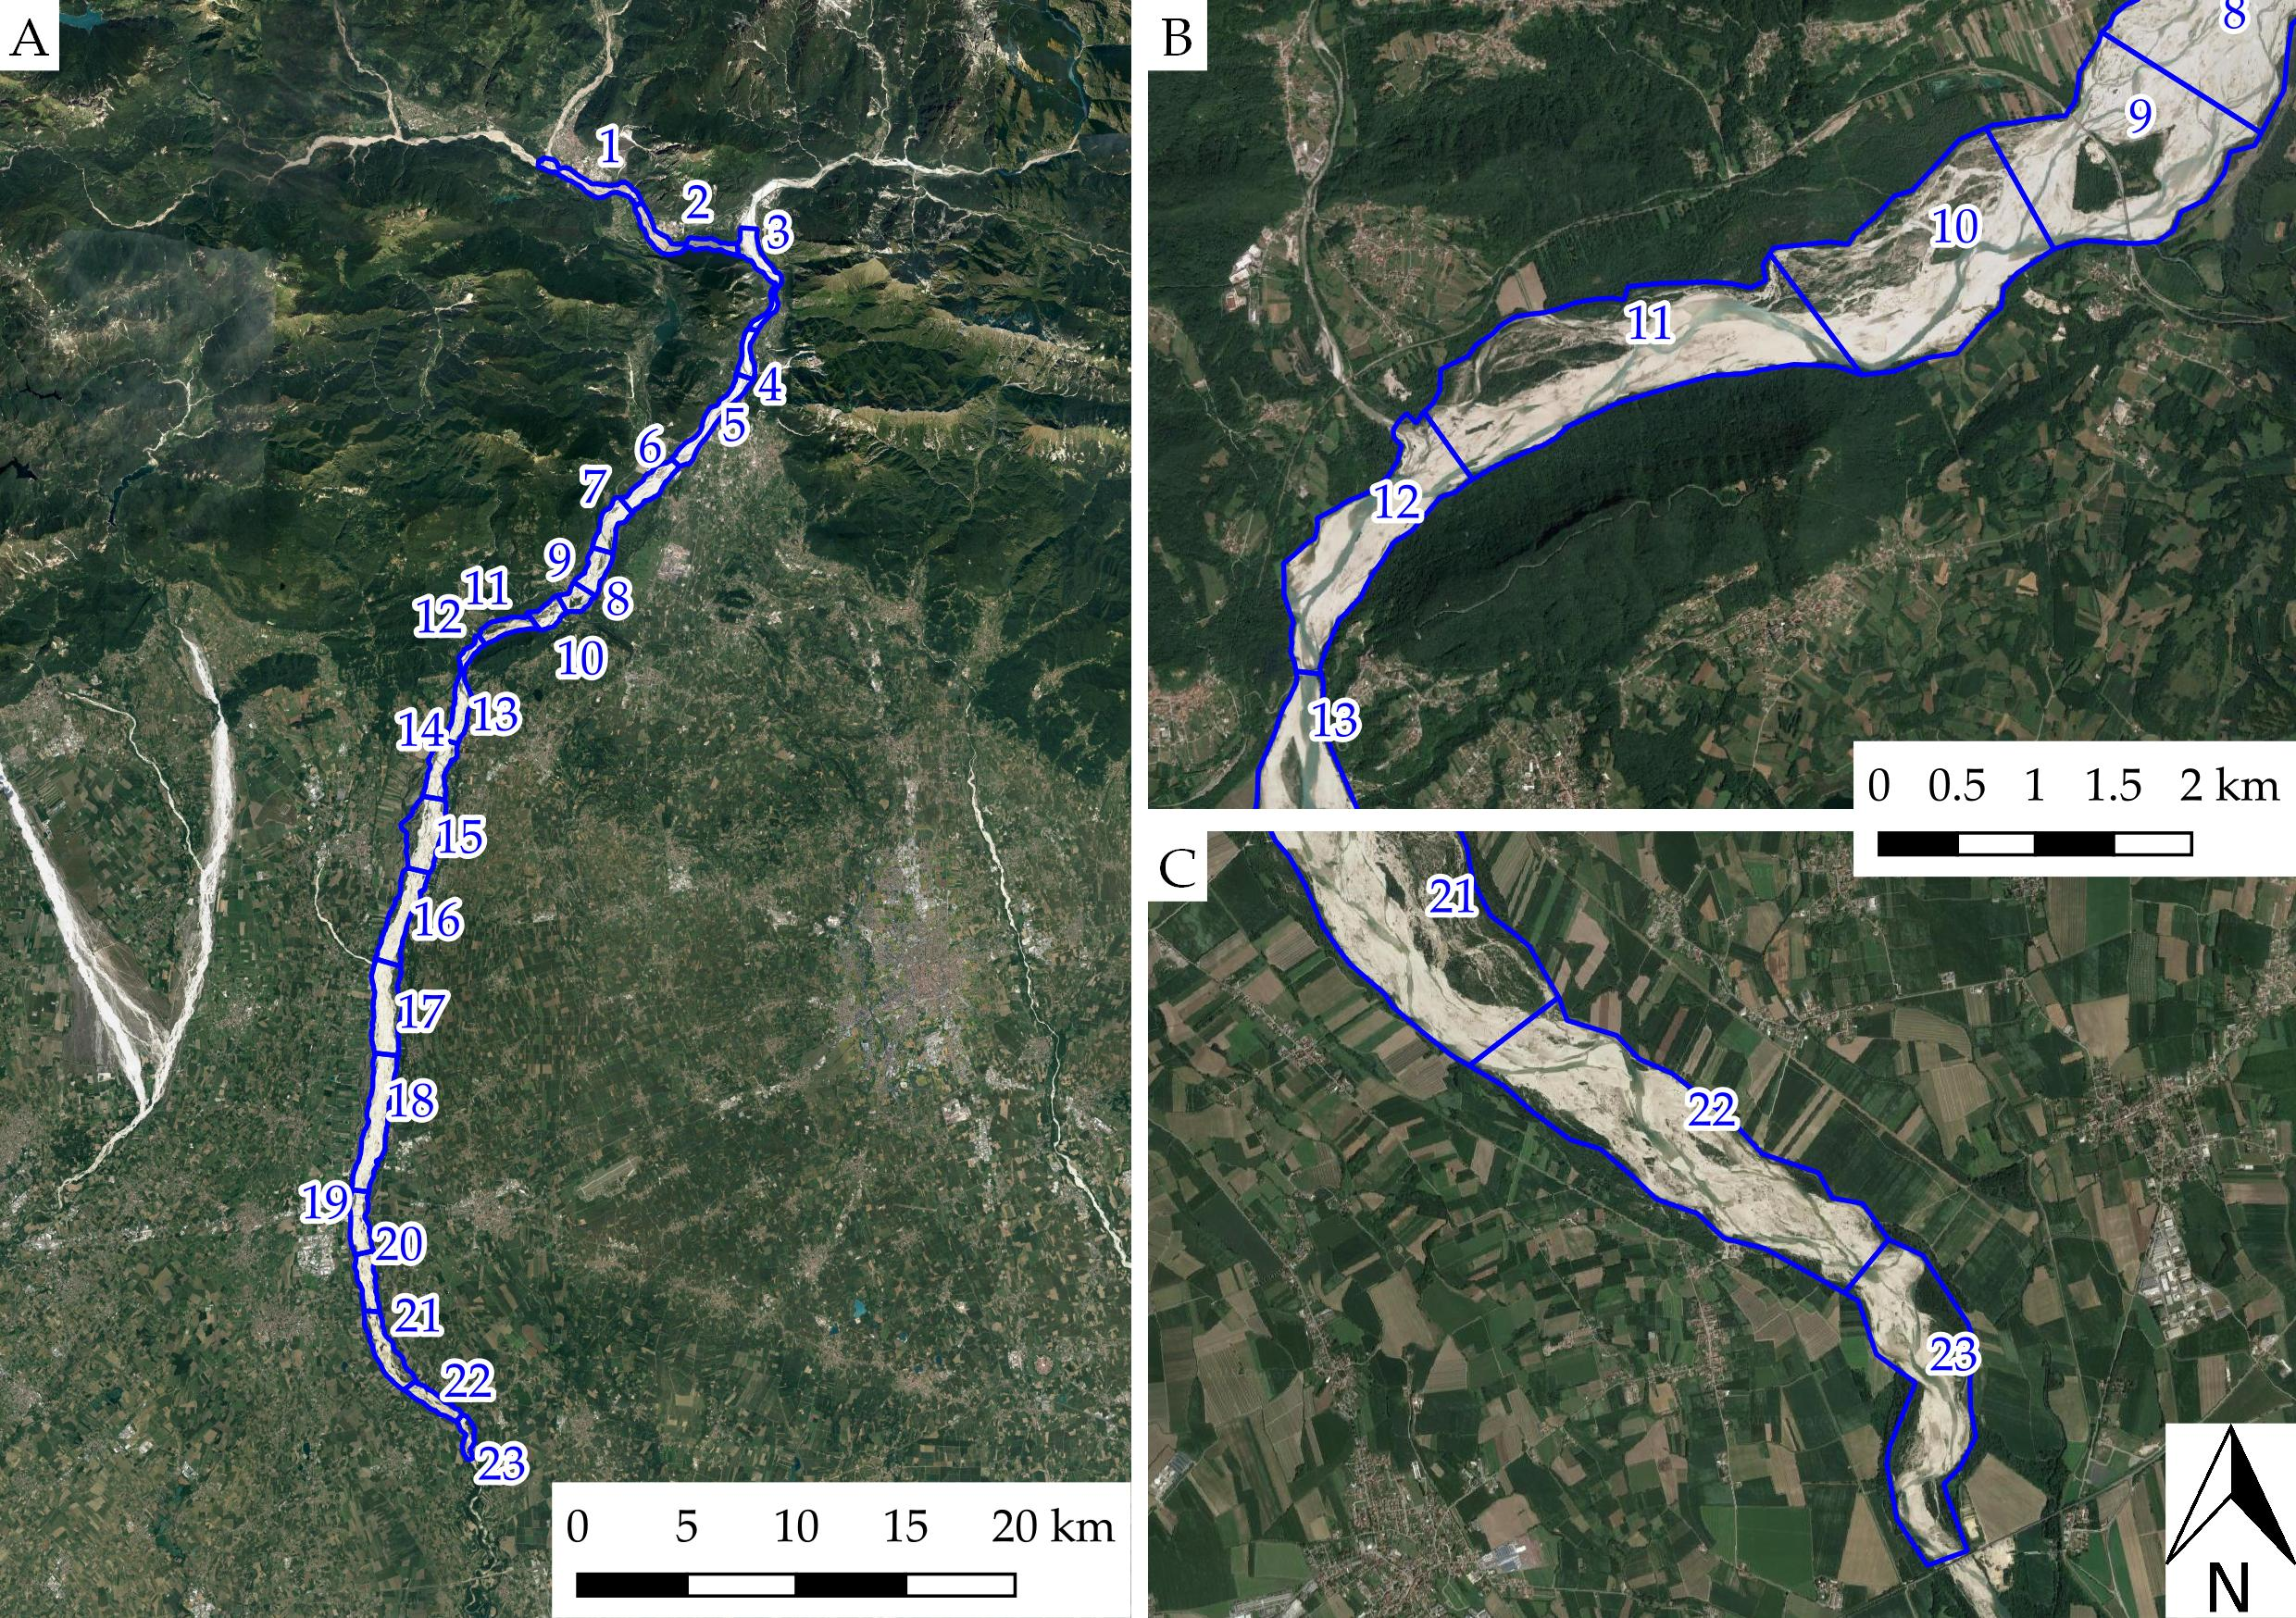
\includegraphics[width=\textwidth]{files/tutti_23_tratti.jpeg}
	\caption[i 23 tratti in cui è suddivisa l'area di studio]{i 23 tratti in cui è suddivisa l'area di studio (figura~A); la sezione di monte del tratto~1 corrisponde a Tolmezzo, la sezione di valle del tratto~23 corrisponde al ponte di Madrisio. A destra sono mostrati ingrandimenti dei tratti presso l'isola di Cornino e la stretta di Pinzano (figura~B) e nei tratti dove la morfologia diventa transizionale poco a monte di Madrisio (figura~C).
	\\
	Map data: Google, Digital Globe.}
	\label{fig:23-tratti}
\end{figure}


\paragraph{Connessione con la falda}
Nel tratto di studio nei pressi del paese di Pinzano al Tagliamento~(PN) è presente una stretta causata dall'affioramento di strati rocciosi che riduce la larghezza da diverse centinaia di metri a circa \SI{130}{\m}.
Questo restringimento, congiuntamente all'innalzamento dello strato di roccia che si trova sotto il letto del fiume, induce variazioni longitudinali nel livello di falda nel materasso alluvionale.
L'acqua filtrante da monte risale in alveo sotto forma di sorgenti diffuse: si assiste al fenomeno dell'\emph{upwelling}.
A valle della stretta, dove l'alveo non è più confinato e il letto roccioso sprofonda nel sottosuolo, l'acqua torna ad infiltrarsi nel materasso ghiaioso (\emph{downwelling}) tanto da portare il fiume in condizioni di secca in certi tratti quando non ci sono piene.
\\
L'\emph{upwelling} e il \emph{downwelling} sono fenomeni rilevanti durante i periodi di magra: certi tratti a valle della stretta di Pinzano possono essere in condizioni di secca, privi completamente di acqua, la quale scorre tutta nel sottosuolo e riemerge presso la “Linea delle risorgive” \squarecite{Mosetti:1983}, quando la morfologia fluviale diventa transizionale pochi chilometri a monte del ponte di Madrisio.
\\
Durante le piene questi fenomeni sono invece irrilevanti: l'acqua che emerge o che si infiltra contribuisce minimamente alla portata fluente.
\\
Il moto di infiltrazione contribuisce al mantenimento di una forte biodiversità caratteristica dell'ambiente fluviale, oltre a permettere una costante purificazione dell'acqua fluente in periodi di magra.

\paragraph{Affluenti}
Nel tratto di studio vi sono diversi affluenti (\cref{fig:affluenti}); vengono qui elencati da monte (Tolmezzo) fino a valle (Madrisio):
%
\begin{itemize}
	\item poco a valle di Tolmezzo c'è il Fella in sinistra idrografica (\SI{706}{\kilo\m\tothe{2}});
	\item all'altezza del paese di Venzone~(UD), in sinistra idrografica, sfocia il torrente Venzonassa (\SI{39}{\kilo\m\tothe{2}});
	\item qualche chilometro a monte del paese di Cornino~(UD) in destra idrografica c'è il Leale (\SI{100}{\kilo\m\tothe{2}}), che ha sempre acqua fluente poiché riceve lo scarico della centrale idroelettrica che sfrutta il lago di Cavazzo; questo raccoglie le acque della parte montana del Tagliamento attraverso opere idrauliche;
	\item in corrispondenza dell'isola di Cornino in sinistra idrografica il Ledra (\SI{75}{\kilo\m\tothe{2}}) riporta nel corso del Tagliamento sia le acque che si sono infiltrate nella piana di Osoppo~(UD) \squarecite{Mosetti:1983} sia quelle intercettate dalla presa di Ospedaletto~(UD);
	\item immediatamente a monte della stretta di Pinzano in destra idrografica si getta l'Arzino (\SI{123}{\kilo\m\tothe{2}});
	\item infine, una decina di chilometri più a valle della stretta in destra idrografica si incontra il Cosa (\SI{160}{\kilo\m\tothe{2}}).
\end{itemize}
%
\begin{figure}
	\centering
	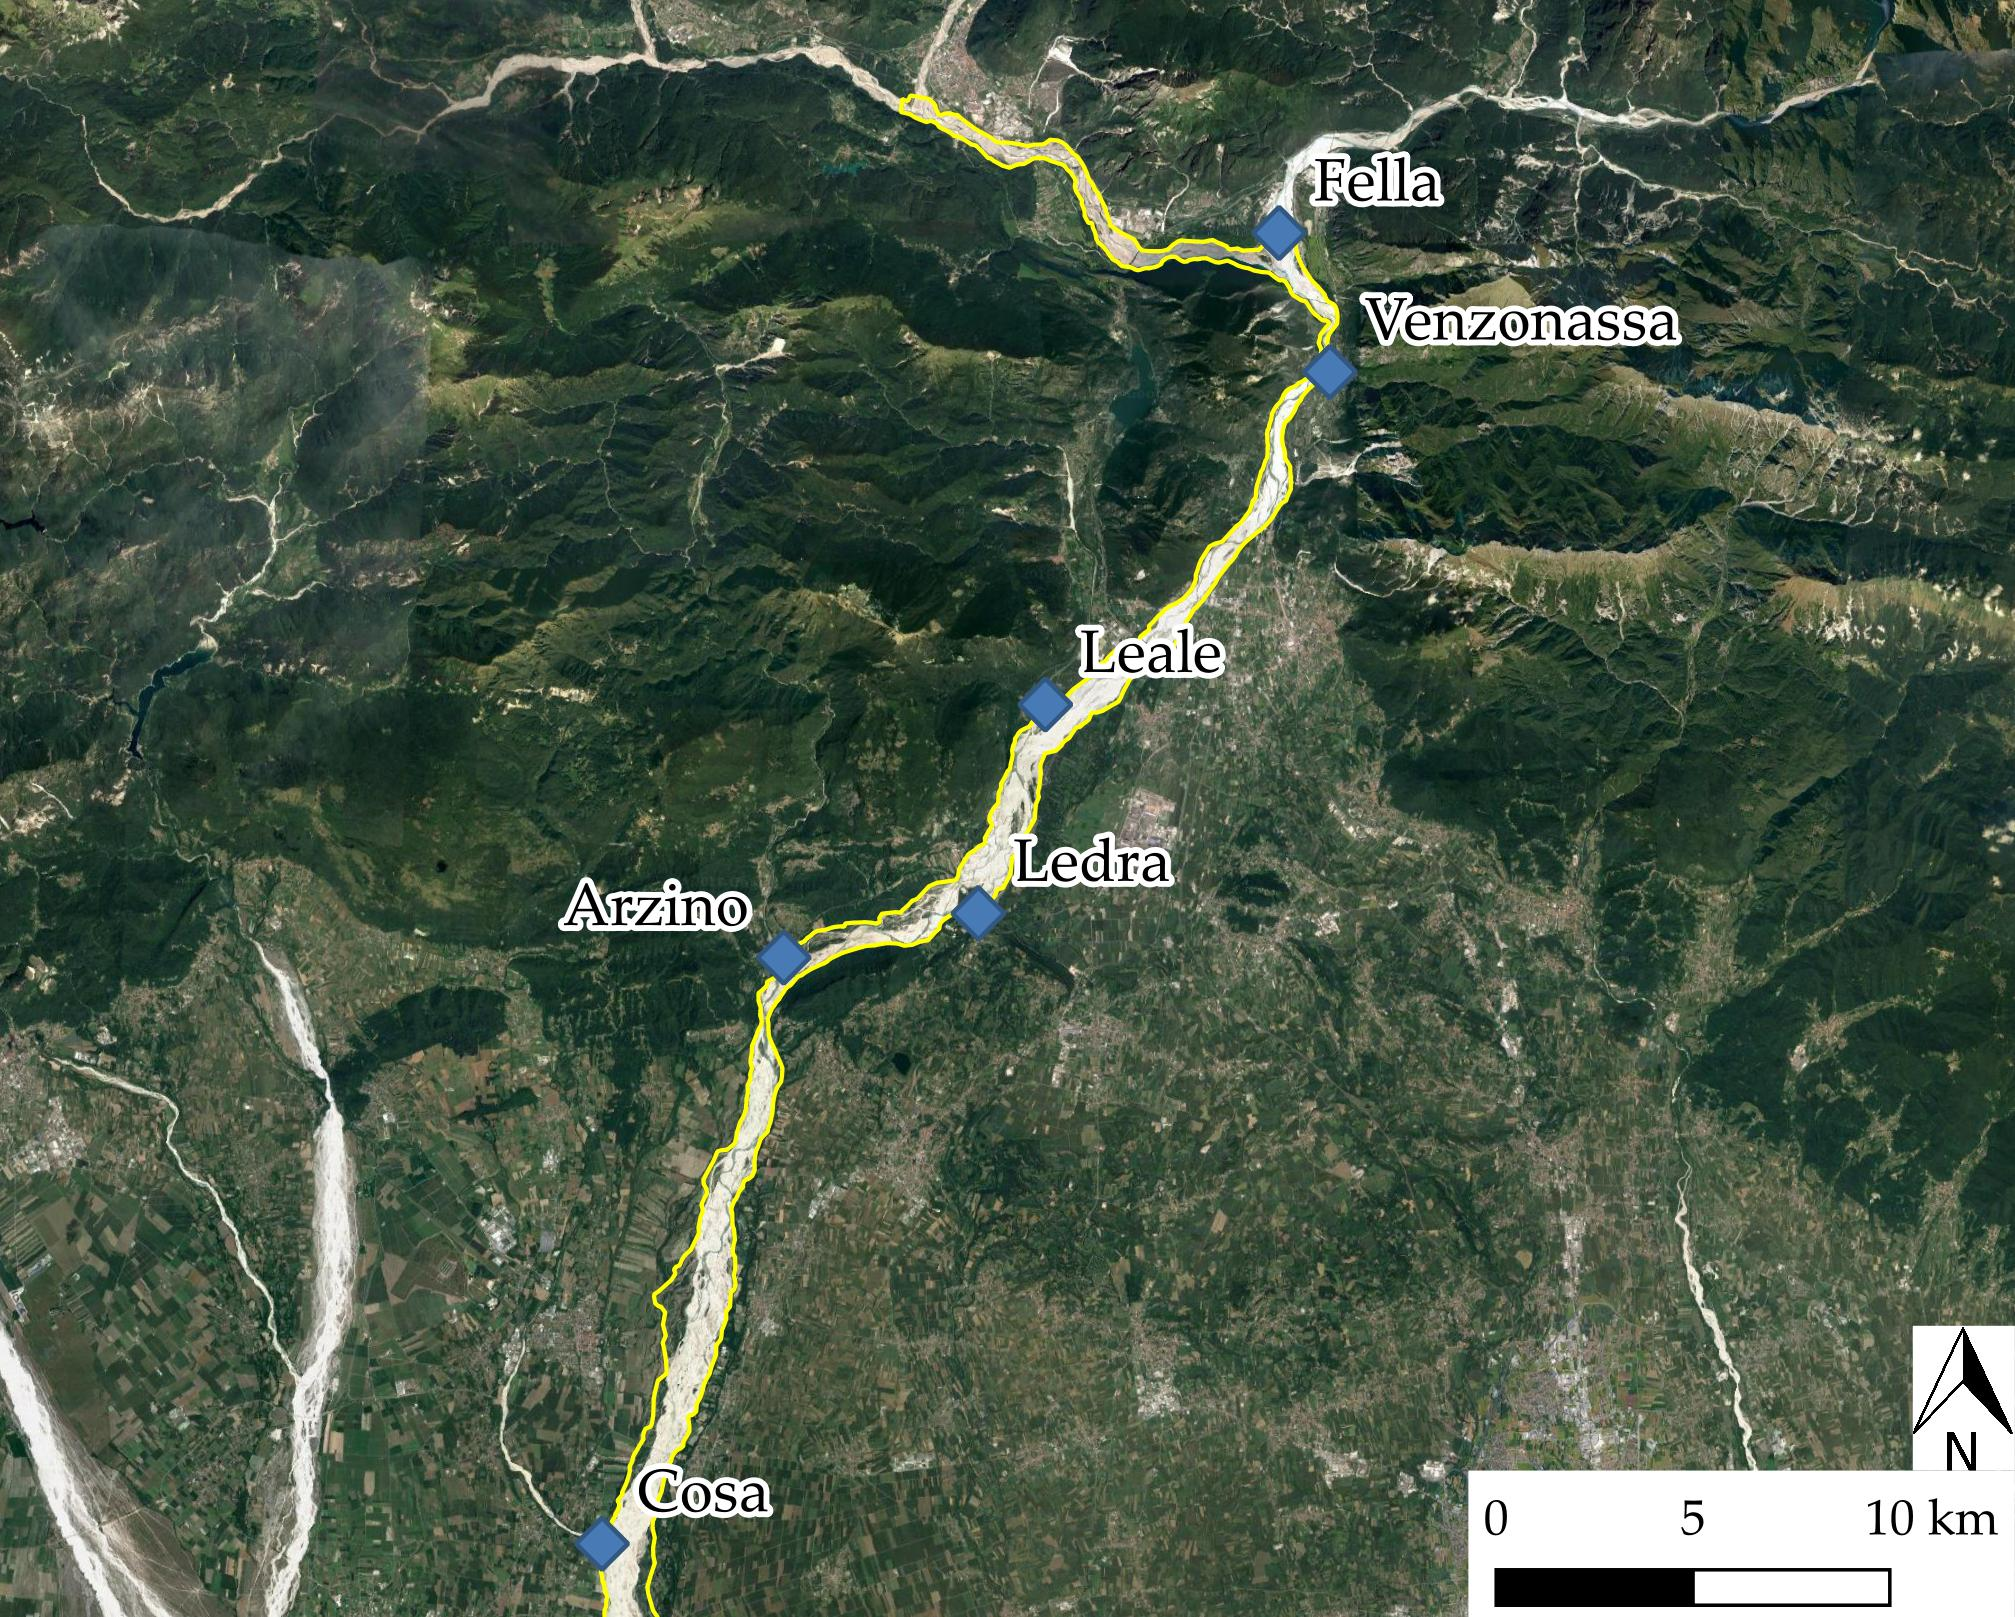
\includegraphics[width=\textwidth]{files/overview_affluenti.jpeg}
	\caption[principali affluenti nel tratto oggetto di studio]{principali affluenti nel tratto oggetto di studio (contornato in giallo).
	\\
	Map data: Google, Digital Globe.}
	\label{fig:affluenti}
\end{figure}
%
Il contributo di questi affluenti in termini di portata non è trascurabile; qualche decennio fa è stata evinta una relazione empirica tra l'area drenante di ogni bacino del Friuli Venezia Giulia \si{[\m\tothe{2}]} e la portata massima registrata in alcuni anni prima del 1950 \si{[\m\tothe{3}\per\s]} \squarecite{Mosetti:1983} che mostra l'evidente importanza degli affluenti:
%
\begin{equation}
	\label{eq:area-portata-mosetti}
	Q = 0.04598 \, A^{0.9546}	\quad	.
\end{equation}
%
Il limite di tale formula risiede nella determinazione delle portate utilizzate per la sua taratura; tuttavia la relazione fornisce la chiara indicazione che la portata in una sezione è all'incirca proporzionale all'area drenante sottesa.
\\
Si ritiene pertanto che conoscere il livello d'acqua in un punto del Tagliamento sia sufficientemente rappresentativo per descrivere qualitativamente l'entità di una piena in tutto il tratto di studio; per ottenere informazioni quantitative sulla portata fluente durante eventi di piena si assume che questa sia proporzionale all'area drenante in ogni sezione del fiume.

\paragraph{Dinamiche vegetazionali}
Nel fiume sono presenti numerose isole, composte prevalentemente da ontani bianchi \emph{Alnus incana} nei tratti montani (oltre l'area di studio), pioppi \emph{Populus nigra} e numerose specie di salice \emph{Salix spp.} nei tratti intermedi e vallivi.
Un'isola è un'area discreta e ben definita dell'alveo ricoperta da vegetazione e circondata da ghiaia o da canali (\cref{fig:esempio-isola}) \squarecites{Gurnell:2001-island-formation}{Bertoldi:2009-2m}.
%
\begin{figure}
	\centering
	\begin{subfigure}[b]{0.37\textwidth}
		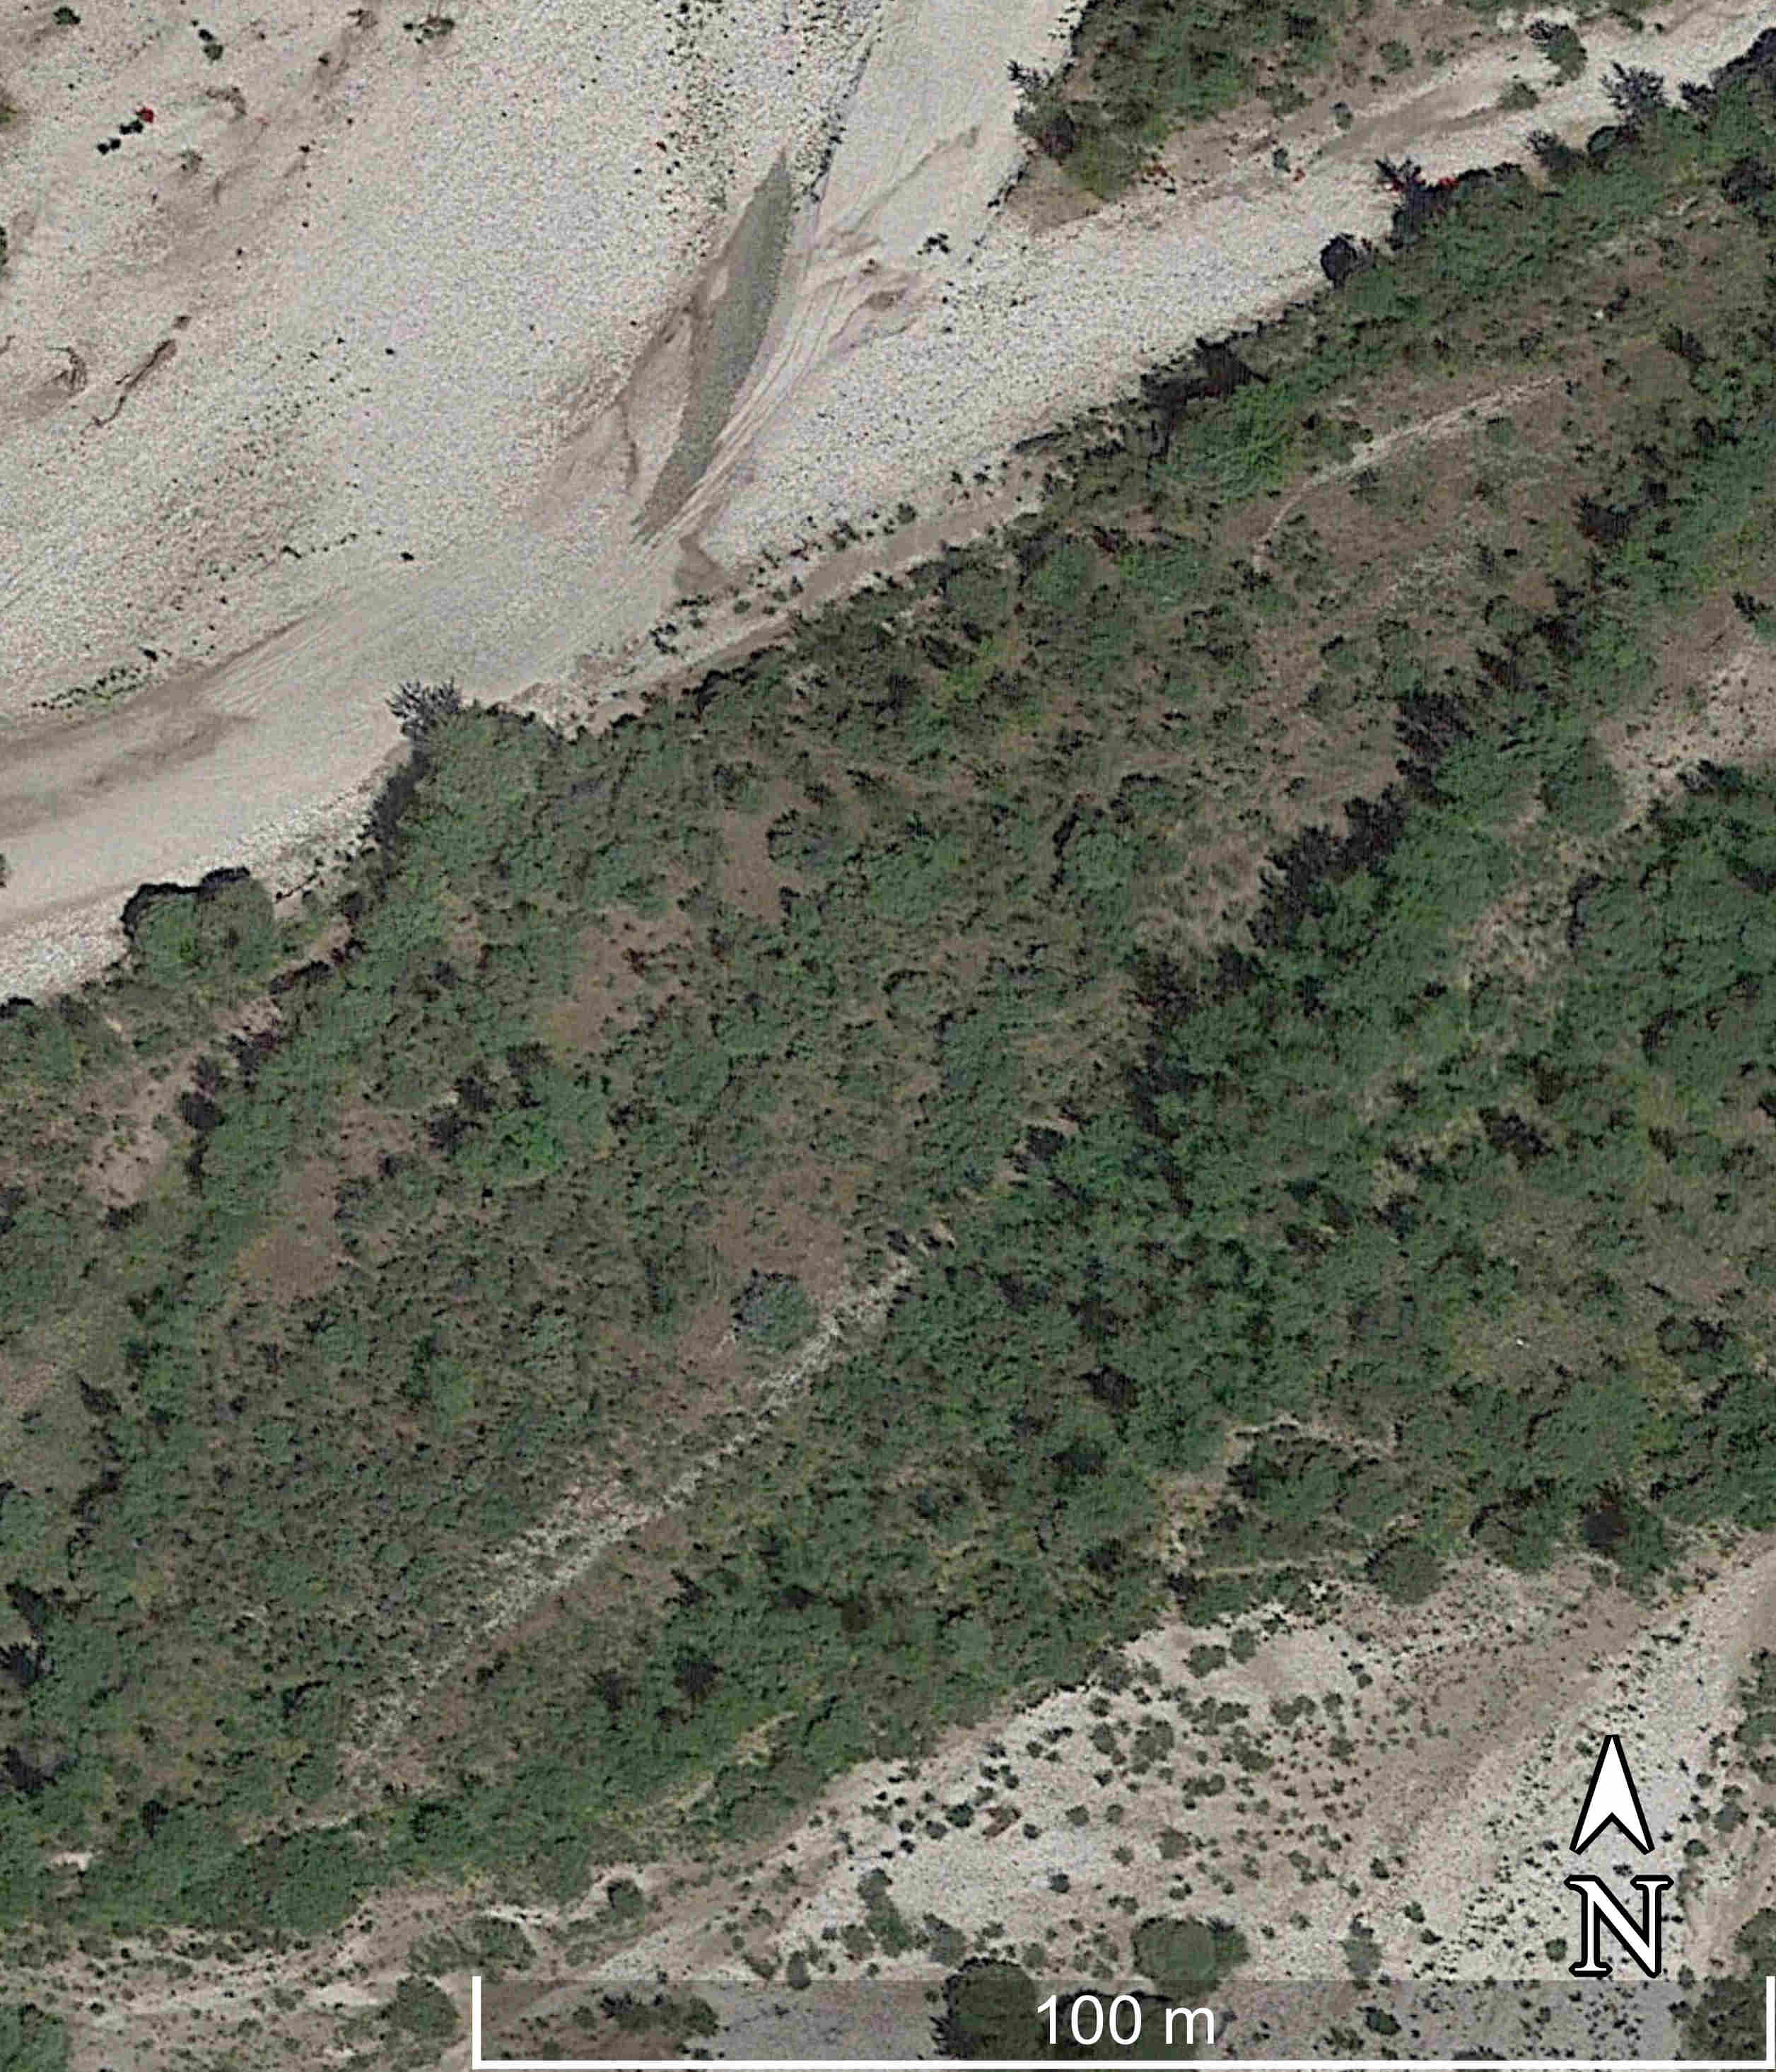
\includegraphics[width=\textwidth]{files/esempio_isola_sat_1.jpg}
	\end{subfigure}
	\quad
	\begin{subfigure}[b]{0.57\textwidth}
		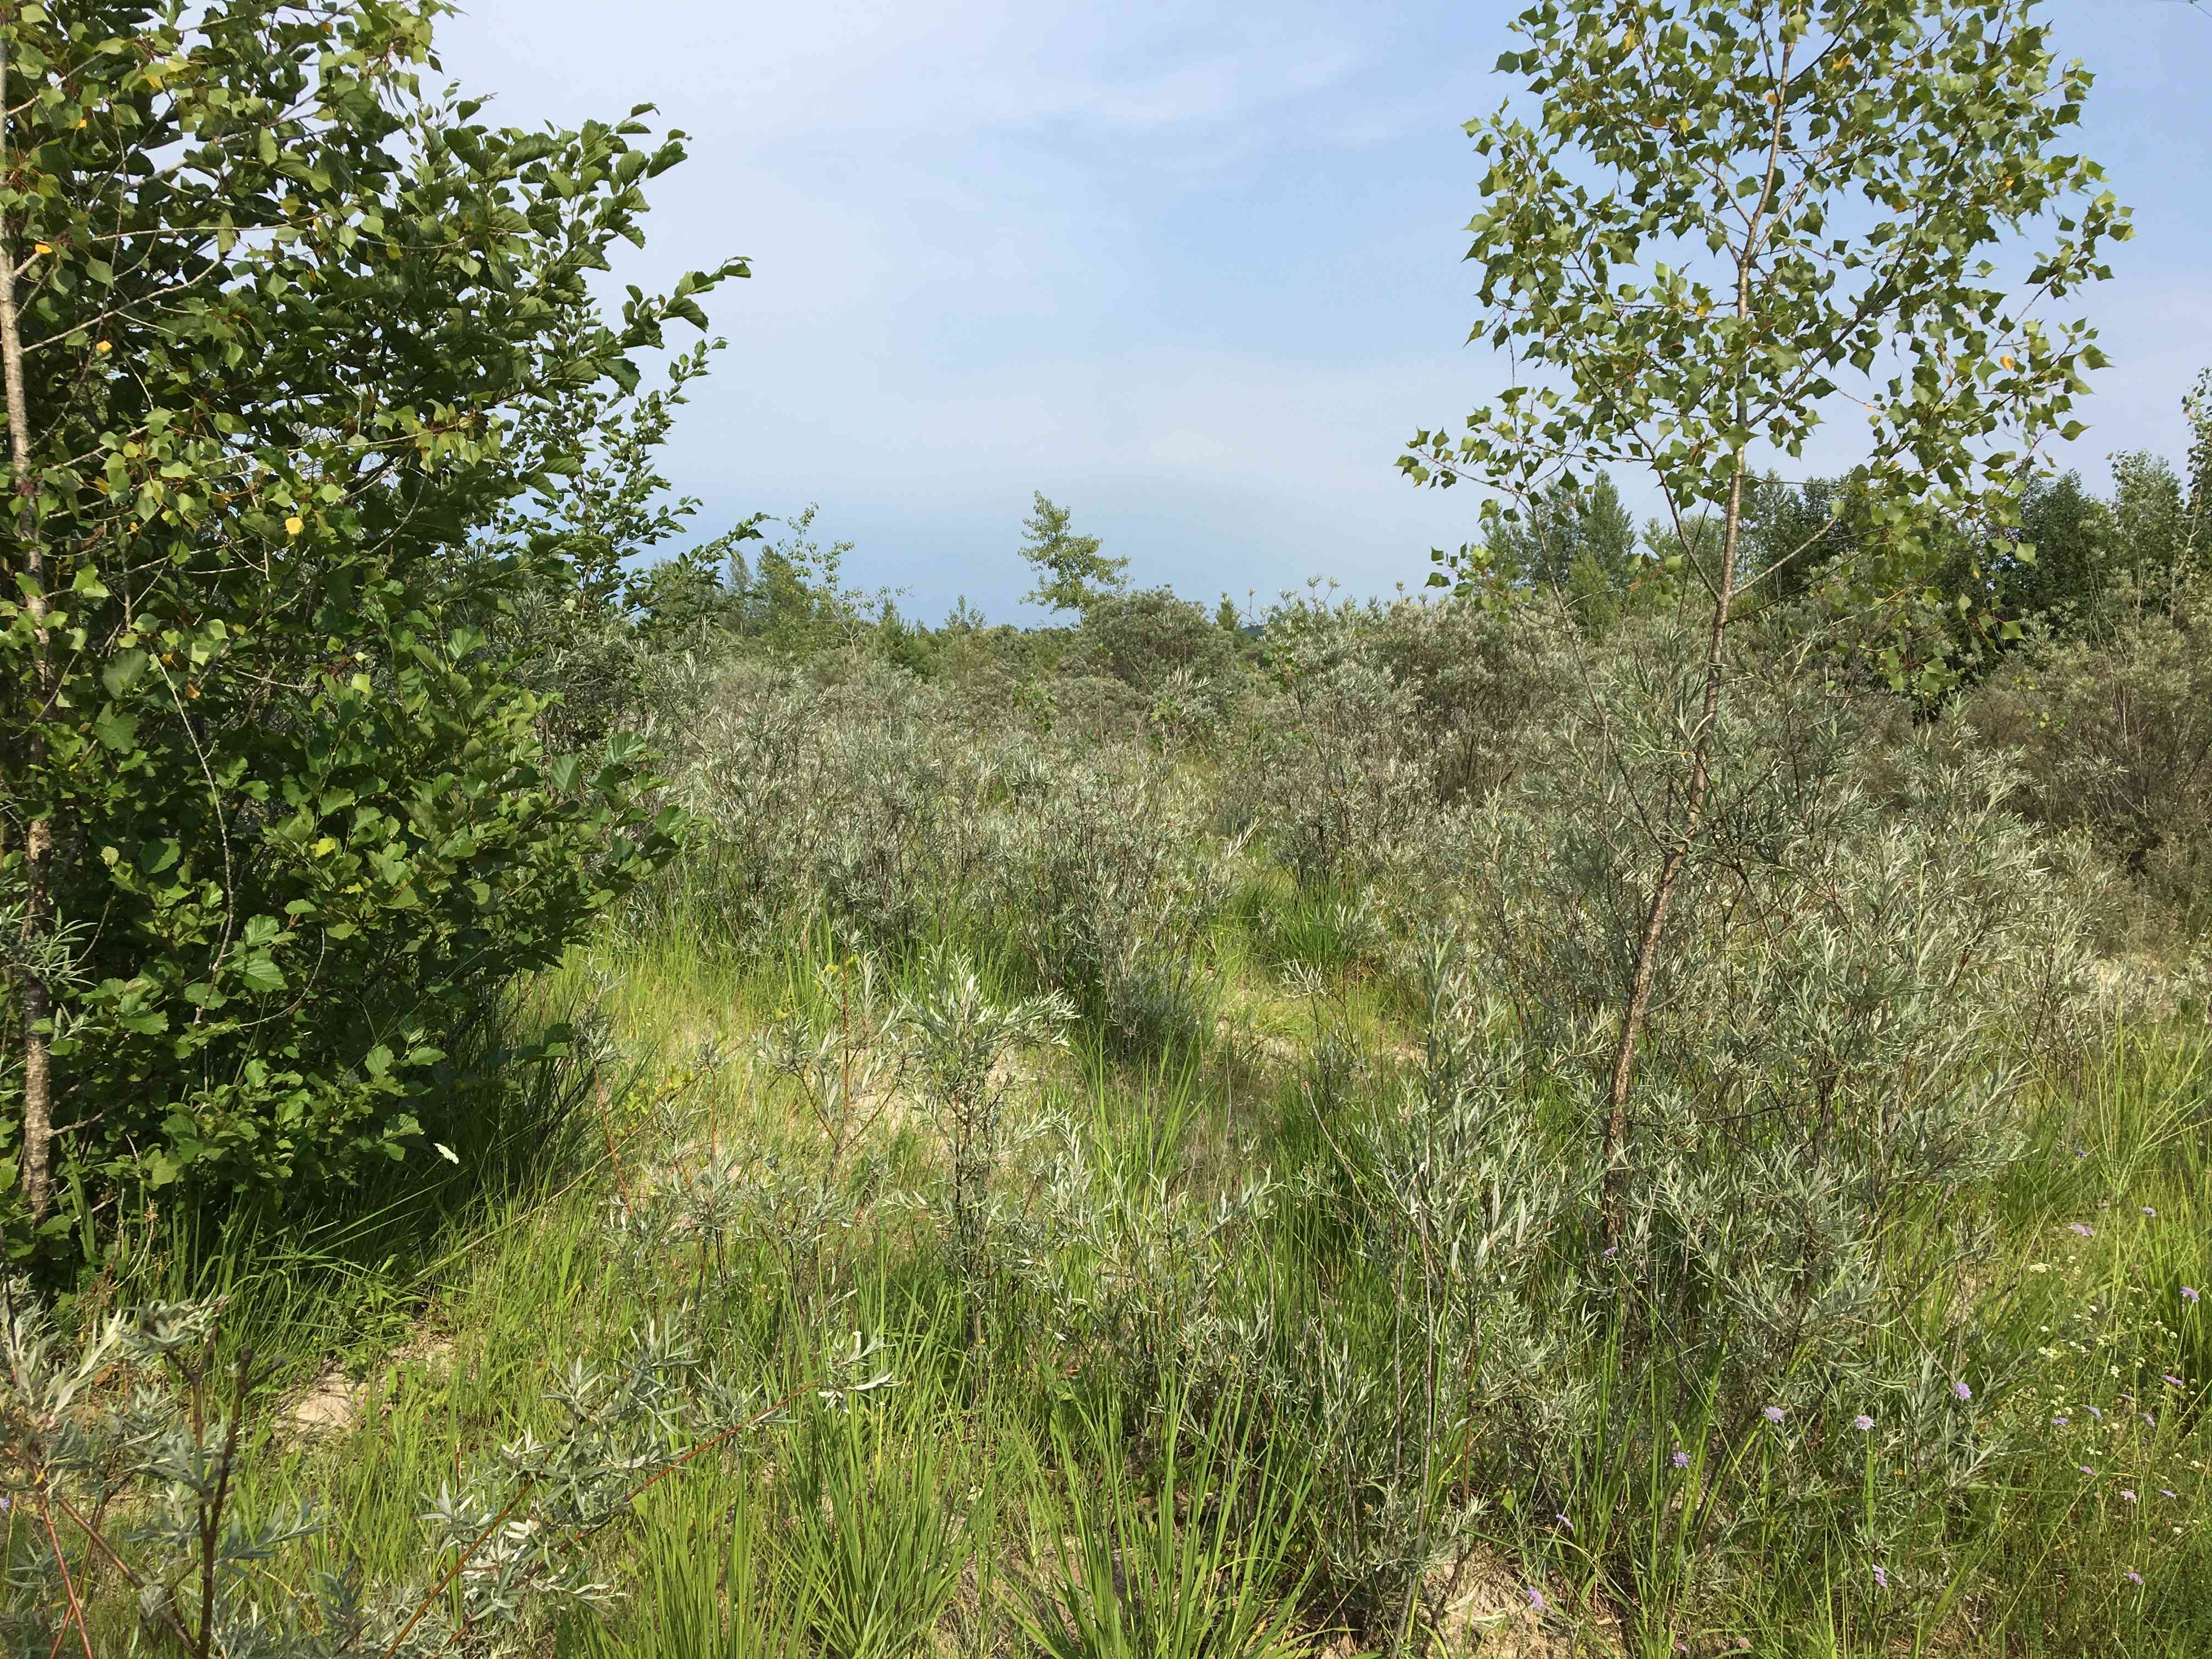
\includegraphics[width=\textwidth]{files/esempio_isola_1.jpg}
	\end{subfigure}
	\caption[immagine e foto di isole fluviali]{immagine da Google Earth e foto di isole fluviali; si noti la forte presenza di salici (\emph{Salix spp.}) e di pioppi (\emph{Populus nigra}); il luogo della foto è prossimo a quello dell'immagine.}
	\label{fig:esempio-isola}
\end{figure}
%
\\
Il meccanismo fondamentale di generazione di forme vegetate in alveo è la ricrescita vegetativa che caratterizza \emph{P. nigra} e \emph{Salix spp.}: i tronchi eradicati e trasportati dalle piene e in seguito depositati sulla nuda ghiaia rigettano rami e foglie (\cref{fig:esempio-accumulo});
se vi è la contemporaneità di adeguate condizioni ambientali (non eccessiva velocità di abbassamento della falda in un substrato di pezzatura adeguata) ed idrologiche (frequenti piene di piccola-media entità, chiamate \emph{flow pulses}) allora i tronchi vivi crescono, intrappolano sedimenti e creano un buon ambiente per la successiva colonizzazione da parte di nuove piante (isole pioniere);
le isole si aggradano (fino a \SI{2}{\m} \squarecite{Gurnell:2006-omega}) e accrescono caratterizzandosi con piante di diversa età (\emph{building island} e isole complesse) \squarecite{Gurnell:2001-island-formation}.
A loro volta la presenza delle isole influenza la posizione, grandezza, forma dei canali e le dinamiche del fondo.
%
\begin{figure}
	\centering
	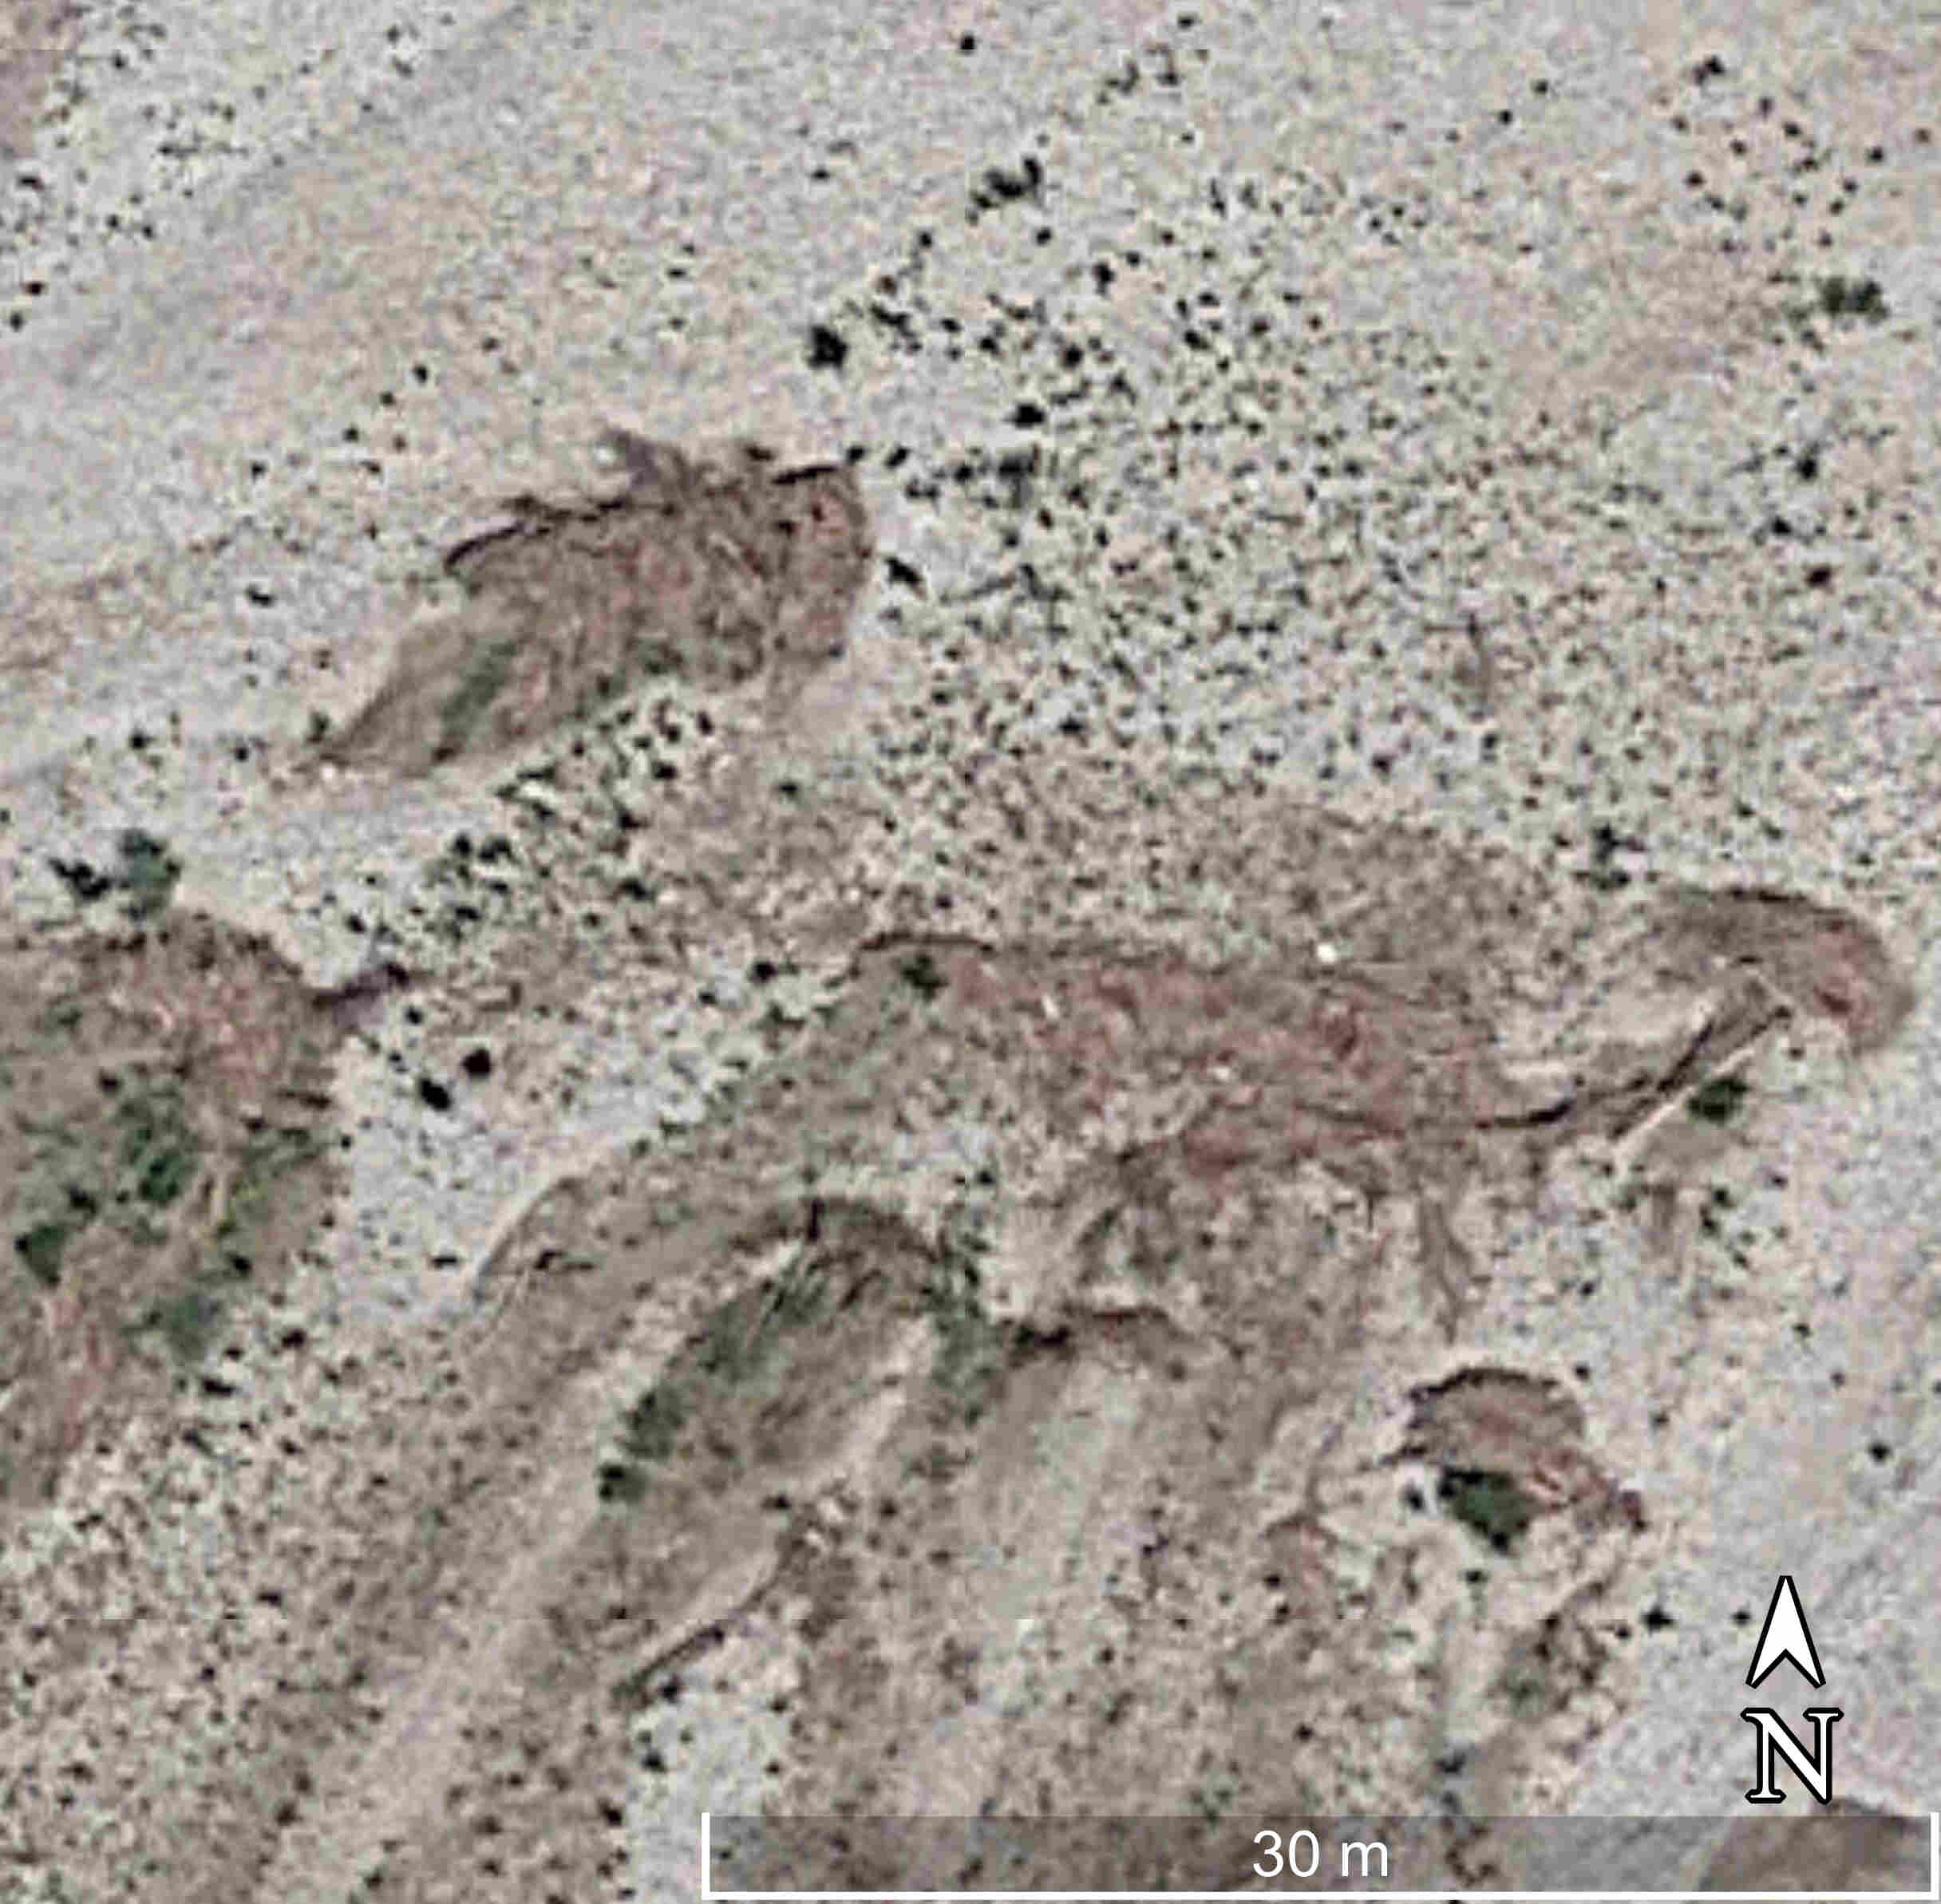
\includegraphics[width = .45\textwidth]{files/esempio_accumulo_sat_1.jpg}
	\quad
	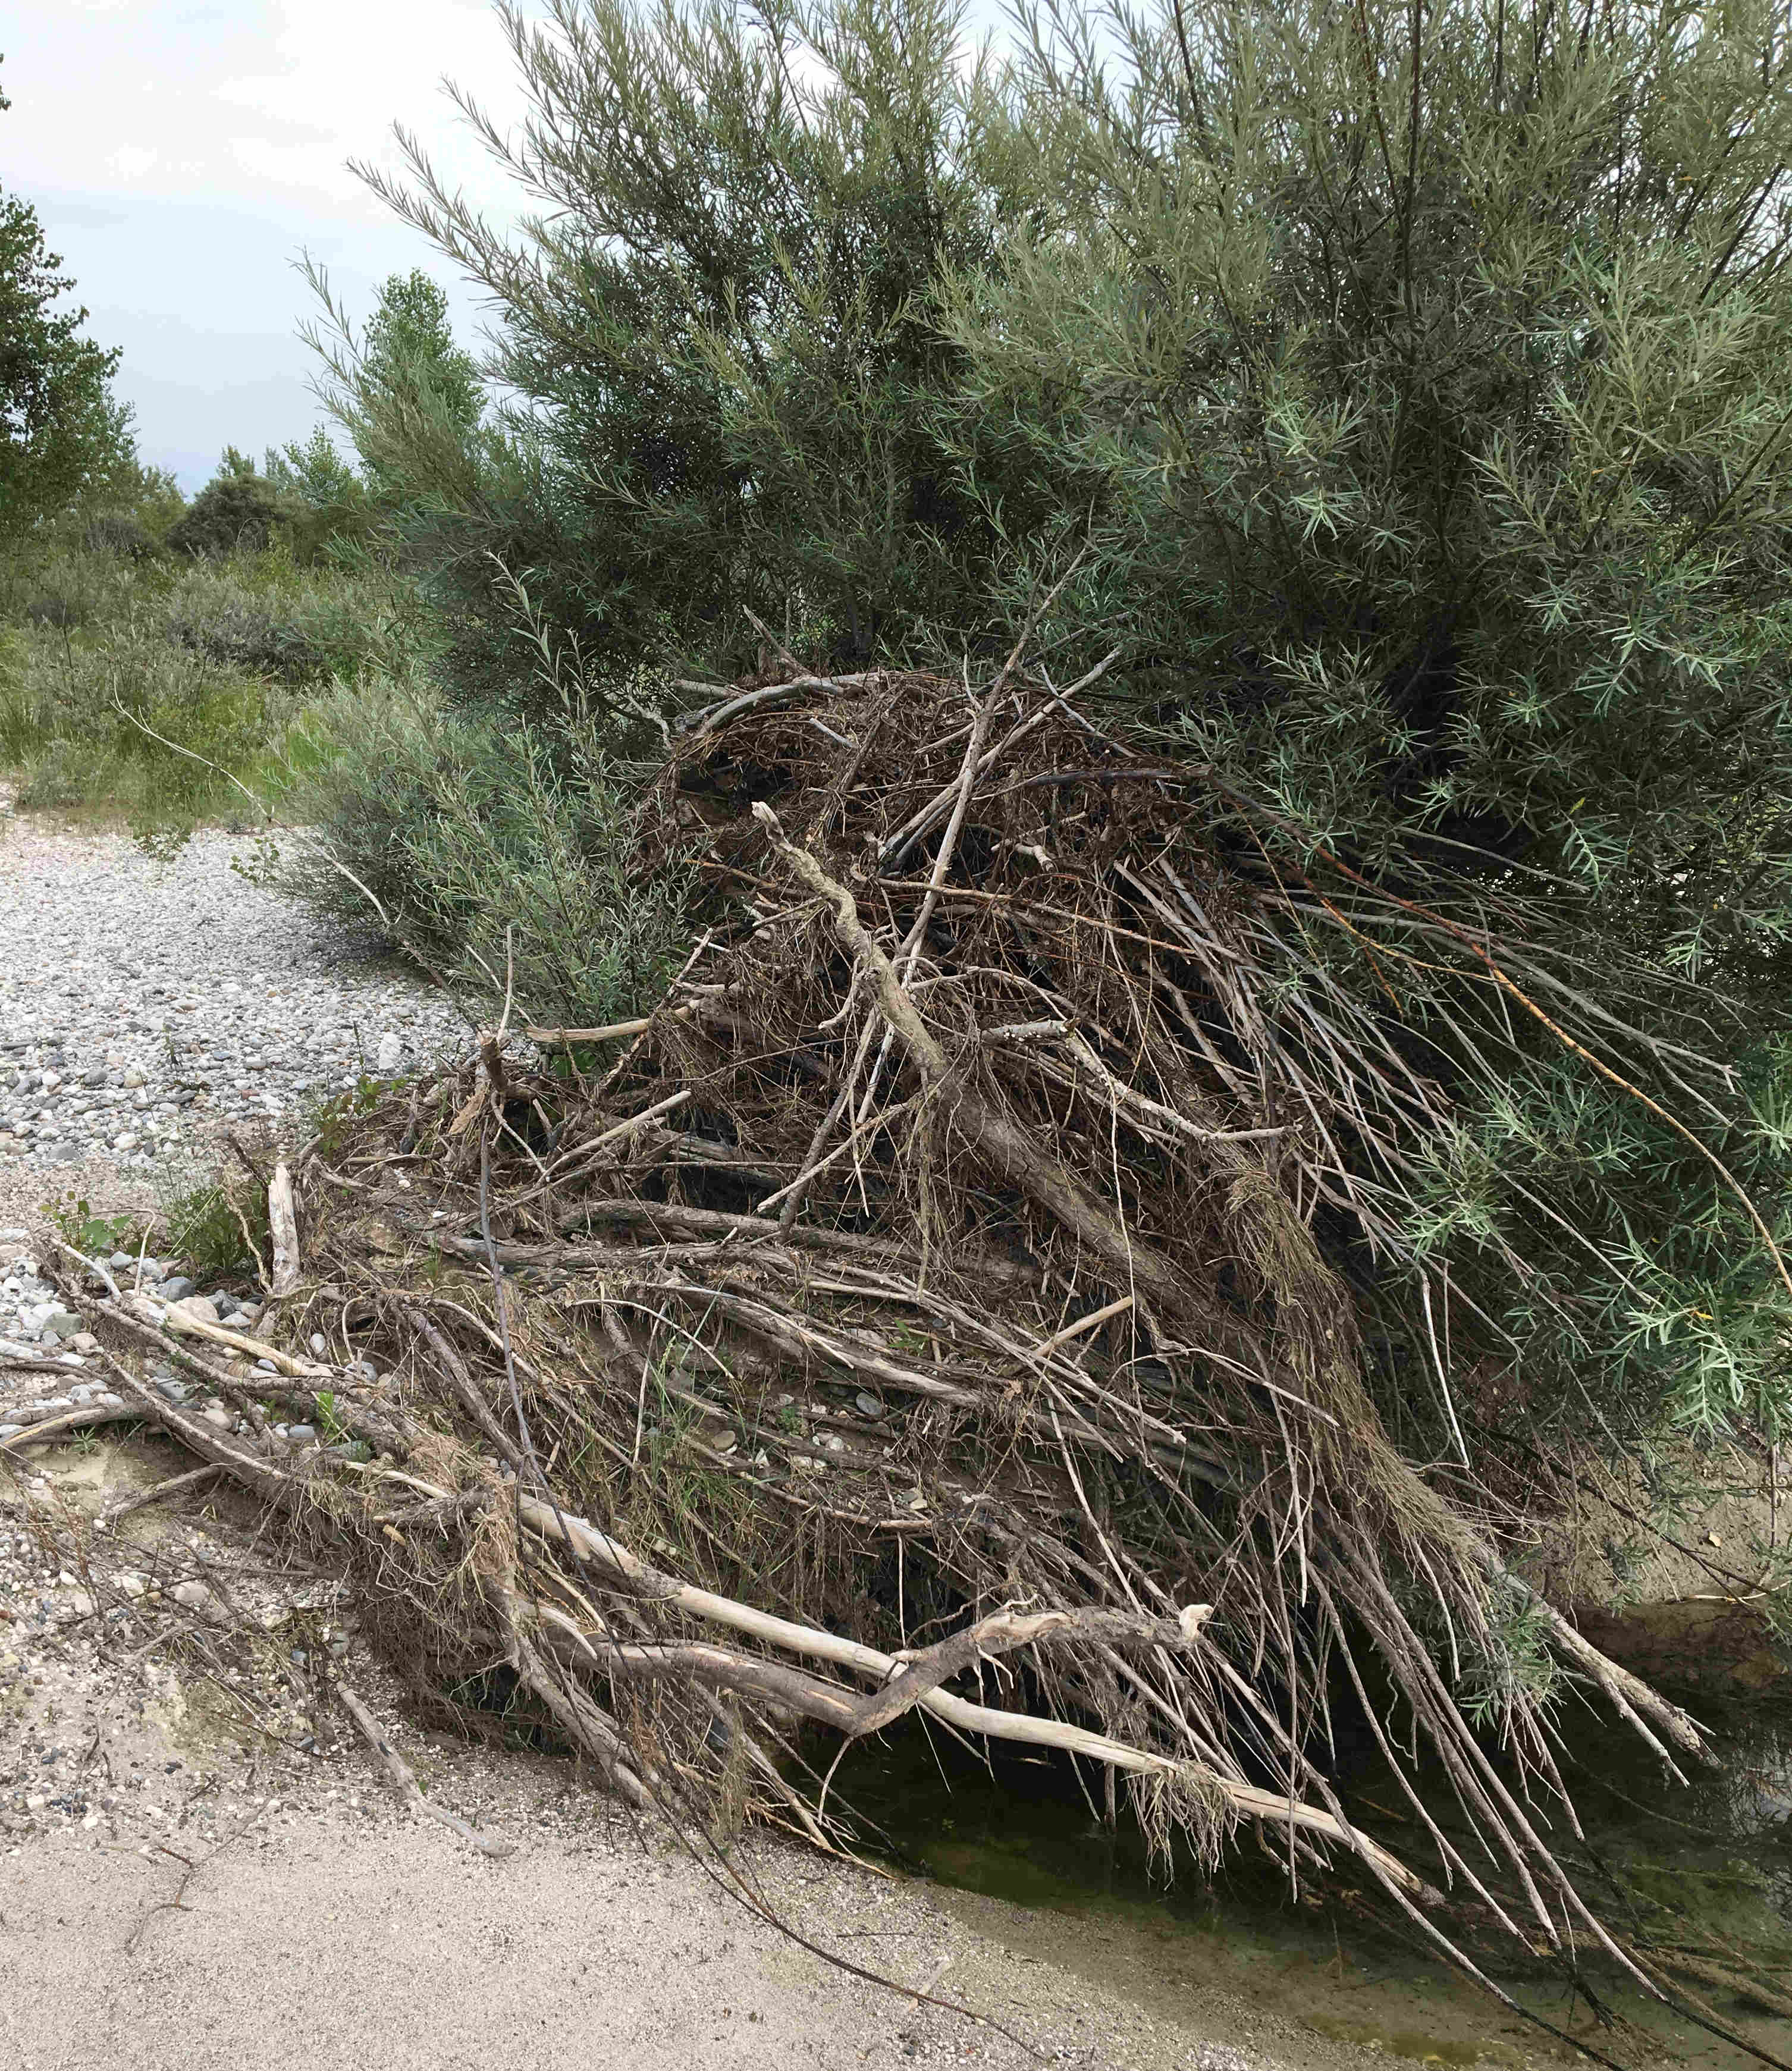
\includegraphics[width = .45\textwidth]{files/esempio_accumulo_1.jpg}
	\caption[immagine e foto di accumuli legnosi]{immagine e foto di accumuli legnosi in grado di rigettare nuovi rami e radici. Il luogo della foto non corrisponde a quello dell'immagine.}
	\label{fig:esempio-accumulo}
\end{figure}
%
\\
Si parla quindi di successione biogeomorfica nel corridoio fluviale attivo: l'ambiente fisico influenza la crescita delle piante coevolute con l'ambiente fluviale; queste a loro volta influenzano l'ambiente fisico e la sua evoluzione, tanto da essere state chiamate “ingegneri ecosistemici” \squarecites{Gurnell:2006-omega}{Gurnell:2014-plants-eng}.

Possono formarsi isole anche da piante nate da seme, anche se queste sono più esigenti in termini di condizioni ambientali ed idrologiche.
\\
Eventi di piena che riempiono l'alveo fino a lambire le sponde (\emph{bankfull}) od eventi più intensi possono dividere parti di vegetazione riparia dalla piana alluvionale, dando origine ad isole composte da piante mature coetanee, strutturalmente ben diverse dalle isole disetanee formate a partire da frammenti vegetativi.

Le isole sono distribuite disomogeneamente da monte verso valle: si può osservare che nei tratti con \emph{upwelling} il loro numero e la velocità di espansione crescono grazie all'acqua che risale dalla falda, mentre nei tratti con \emph{downwelling} la loro presenza diminuisce;
inoltre, nelle zone particolarmente più strette come nei tratti montani o presso la stretta di Pinzano l'intensità della corrente è tale da ridurre o inibire la crescita di vegetazione, come mostrato da un modello concettuale in letteratura \squarecite{Gurnell:2014-plants-eng}.
\\
Temporalmente, le uniche isole che non vengono erose sono quelle che si fondono nella piana alluvionale; anche isole insediatesi da anni in alveo, aggradatesi fino a porsi a quote simili a quelle della \emph{floodplain}, possono essere completamente spazzate durante eventi \emph{bankfull} o maggiori.
Difatti è stato mostrato che la maggior parte delle isole nel tratto compreso tra il ponte autostradale di Braulins e la stretta di Pinzano persistono meno di \SI{24}{\anni} \squarecite{Zanoni:2008}; risultati simili sono stati presentati per un tratto nei pressi di San Paolo~(PN), corrispondente ai tratti più a valle nella presente tesi \squarecite{Bertoldi:2009-2m}.

L'isola presente nel tratto~9 (\cref{fig:23-tratti}), nei pressi di Cornino, si fonda su un nucleo roccioso.
Questa isola non è soggetta alle dinamiche tipiche delle isole che crescono sulla ghiaia dell'alveo: nemmeno le piene più intense possono asportarla od eroderla parzialmente.


\section{Stato dell'arte ed obiettivi}
\label{sec:stato-arte-obiettivi}
L'obiettivo principale della presente tesi è lo studio delle dinamiche delle isole nel Tagliamento in risposta al regime idrologico (successione di magre, morbide, piene) e la comprensione dei fattori che controllano le traiettorie evolutive della vegetazione.
In via previsionale si cerca di rispondere all'esigenza di stimare in anticipo gli effetti che una piena può avere sulle isole, risultato che aiuterebbe anche a migliorare la gestione dei fiumi e della vegetazione presente in essi in altri contesti dove le portate sono regolate dall'uomo. 
\\
Lo studio è stato effettuato su un periodo di 18~anni, dal~2000 al~2018, analizzando dati telerilevati con tecniche diverse (immagini satellitari, foto aeree, rilievi aerei topografici LiDAR).
I dati così ottenuti sono stati messi in relazione al regime idrologico dello stesso periodo, caratterizzato dalle misure idrometriche di livello del pelo libero presso la stazione di Villuzza~(UD). 

Articoli precedentemente pubblicati hanno studiato l'ecologia e la morfodinamica del Tagliamento, le interrelazioni tra piante e fiume, la crescita della vegetazione riparia, la localizzazione delle isole in questo contesto naturale e molto altro.
\\
Alcuni lavori si sono basati su immagini aeree e indagini di campo \squarecites{Zanoni:2008}{Bertoldi:2010-d50}{Surian:2015}: da una parte questi permettono la raccolta di informazioni in grande dettaglio, ma con risoluzione spaziale modesta (i rilievi aerei hanno un costo non indifferente) e risoluzione temporale particolarmente limitata (da pochi anni a decenni tra ogni rilievo).
\\
L'utilizzo di immagini satellitari multitemporali a bassa risoluzione permette di avere una visione d'insieme dei fenomeni, così come di evidenziare differenze spaziali e temporali.
Infatti è già stato dimostrato che è possibile estrarre risultati significativi sulla vegetazione riparia e sulle sue dinamiche da immagini satellitari a bassa risoluzione \squarecites{Bertoldi:2011-ASTER}{Henshaw:2013-LandSat}.
Questi lavori tuttavia hanno utilizzato delle maschere fisse per delimitare l'area attiva, senza distinguere in ogni immagine le isole dalla \emph{floodplain}.
\\
Alcuni autori hanno inoltre formulato modelli concettuali sulle dinamiche vegetazionali nei fiumi, in particolare nel Tagliamento \squarecites{Gurnell:2001-island-formation}{Gurnell:2006-omega}{Gurnell:2014-plants-eng}.
\\
Generalmente, il tratto più frequentemente studiato è quello compreso tra il ponte autostradale di Braulins~(UD) e la stretta di Pinzano.

Con la presente tesi si vuole provare a rispondere alle seguenti domande, anche grazie ai risultati ottenuti in lavori precedenti.
%
\paragraph{Quante isole sono presenti e cosa ne regola la presenza?}
La larghezza media dell'alveo e la percentuale di isole rispetto all'alveo attivo sono state due grandezze studiate per caratterizzare spazialmente e temporalmente il Tagliamento:
%
\begin{itemize}
	\item il tracciamento della traiettoria evolutiva della larghezza ha permesso di vedere come il tratto a monte di Pinzano si sia ristretto negli ultimi due secoli di più del \SI{50}{\percent}, mentre a partire dalla fine del~1900 sembra che l'alveo abbia ripreso un processo di allargamento \squarecites{Zanoni:2008}{Surian:2015};
	gli autori suggeriscono che il restringimento possa essere dovuto alla concomitanza di lievi cambiamenti naturali nel regime delle portate e per l'estrazione di ghiaia dall'alveo per scopi civili negli anni '70 e '80 del secolo scorso, come è avvenuto per altri fiumi simili \squarecite{Sitzia:2016-d50};
	le cause dell'allargamento possono essere il veto all'estrazione della ghiaia congiuntamente ad un periodo caratterizzato da piene intense nei primi anni del 2000;
	%
	%
	\item la proporzione tra isole e alveo attivo è stata considerata da più autori \squarecites{Zanoni:2008}{Bertoldi:2011-ASTER}{Henshaw:2013-LandSat}{Surian:2015}; 
	mentre alcuni risultati sembrano mostrare un rapporto oscillante attorno ad un valore medio di \SI{8}{\percent} \squarecite{Zanoni:2008}, altri mostrano valori abbastanza diversi come ordine di grandezza \squarecite{Henshaw:2013-LandSat} (probabilmente dovuti all'utilizzo di immagini satellitari con celle di \SI{30}{\m}) o con un trend temporale opposto rispetto alla larghezza \squarecite{Surian:2015}.
\end{itemize}	
%
In un modello concettuale presentato pochi anni fa viene proposta la potenza della corrente come fattore che regola la presenza delle isole \squarecite{Gurnell:2006-omega}: se la corrente ha mediamente un'elevata energia per unità di larghezza, allora la crescita delle piante è inibita; se la potenza è inferiore ad una soglia individuata dagli autori, allora la formazione ed espansione delle isole è controllata da altri fattori ambientali, come la quota della falda e la granulometria del substrato dove crescono le piante.

Con i dati di questa tesi è possibile estendere al periodo presente i risultati e le osservazioni effettuate dagli altri autori sulla larghezza e sulla proporzione di isole rispetto all'alveo attivo, così come sfruttare la maggior risoluzione temporale delle immagini per osservare cambiamenti avvenuti in periodi più brevi.
\\
Inoltre, si cerca non solo di verificare l'esistenza di un valore limite della potenza della corrente oltre il quale non crescono più isole, ma di capire se e in che misura questo fattore può influenzare la massima proporzione di isole presenti in alveo.

\paragraph{In quali condizioni e in quale misura cambiano le isole?}
Le isole sono soggette a continue dinamiche di erosione in seguito alle piene e di accrescimento nei periodi tra un evento e quello successivo.
\\
Diversi autori hanno considerato la persistenza media delle isole nell'alveo, dell'ordine di una ventina d'anni; gli stessi hanno quantificato anche la percentuale di isole erose e le nuove aree vegetate \squarecites{Zanoni:2008}{Bertoldi:2009-2m}{Bertoldi:2011-ASTER}{Surian:2015}.
Tuttavia in alcuni lavori la risoluzione temporale è particolarmente bassa (un'immagine ogni decina di anni), in altri il periodo di studio limitato a pochi anni; in tutti il tratto studiato era quello menzionato all'inizio della sezione, lungo circa~\SI{20}{\kilo\m}.
Si può quindi cercare di migliorare ed ampliare questi risultati sia da un punto di vista spaziale che temporale.
\\
La riproduzione vegetativa a partire da tronchi vivi depositati in alveo è uno dei principali meccanismi di formazione delle isole nel Tagliamento \squarecite{Gurnell:2001-island-formation}. 
Grazie alle ortofoto e alle immagini satellitari ad alta risoluzione si può osservare quanto legno è presente in alveo; con i rilievi LiDAR  si può controllare se gli elementi legnosi che non vengono mobilitati dalle piene sono quelli posti a quote relative maggiori; infine, si può cercare quanti tronchi e accumuli legnosi crescono fino a formare nuove isole.

\paragraph{È utile analizzare l'età delle isole?}
Alcuni autori hanno mostrato come la vegetazione riparia delle isole possa avere una diversa struttura di età in base alle modalità di accrescimento e come le piante mature possano essere generalmente più resistenti all'erosione di piante allo stadio iniziale della successione biogeomorfica \squarecites{Gurnell:2001-island-formation}{Gurnell:2014-plants-eng}.
\\
Ad oggi, tuttavia, sembra che nessun autore abbia provato a caratterizzare l'età della vegetazione nelle isole per migliorare risultati riguardo le dinamiche delle isole.
\\
Con questa tesi si prova ad implementare la divisione della vegetazione nelle isole in classi di età e a verificare se e quanto i risultati ne vengono influenzati: sono le piante più giovani quelle che possono essere erose più facilmente?

\paragraph{Qual è la relazione tra regime delle piene e dinamiche delle isole?}
Precedentemente è già stata formulata una relazione tra isole erose e portata \squarecite{Surian:2015};
questa tuttavia è basata su una piccola quantità di dati e non tiene conto dell'invecchiamento della vegetazione tra piene successive, fattore interessante poiché si potrebbe osservare un'erosione differenziata tra isole appena formatesi e isole insediate in alveo da anni.
\\
Riguardo l'accrescimento, al momento attuale non sono noti all'autore lavori che mettano in relazione la crescita della vegetazione con il periodo che intercorre tra piene successive.

\section{Convenzioni}
Le seguenti convenzioni saranno utilizzate nella presente tesi:
\begin{description}
	\item[Capitoli] riprendono le domande formulate nella sezione~\ref{sec:stato-arte-obiettivi}; ogni sezione di risposta è suddivisa in metodi (quali tecniche sono state utilizzate e quali analisi sono state svolte), risultati (cosa è possibile osservare oggettivamente dai dati) e discussione (quale interpretazione è possibile dare ai risultati);
	\item[Mappe] riportate secondo WGS84/UTM~33N (EPSG:~32633);
	\item[Direzione della corrente] riportata con una freccia blu nelle immagini;
	\item[Formato delle date] AAAA-MM-GG;
	\item[Citazioni] sono nel formato Autore/i-Anno, racchiuse tra parentesi quadre;
	\item[Web link] sono riportati in note a piè pagina;
	\item[Termini in lingua straniera] sono in corsivo;
	\item[Glossario] presente nel materiale finale.
	%
\end{description}

